%% abtex2-modelo-trabalho-academico.tex, v-1.7.1 laurocesar
%% Copyright 2012-2013 by abnTeX2 group at http://abntex2.googlecode.com/
%%
%% This work may be distributed and/or modified under the
%% conditions of the LaTeX Project Public License, either version 1.3
%% of this license or (at your option) any later version.
%% The latest version of this license is in
%%   http://www.latex-project.org/lppl.txt
%% and version 1.3 or later is part of all distributions of LaTeX
%% version 2005/12/01 or later.
%%aa
%% This work has the LPPL maintenance status `maintained'.
%%
%% The Current Maintainer of this work is the abnTeX2 team, led
%% by Lauro C\'{e}sar Araujo. Further information are available on
%% http://abntex2.googlecode.com/
%%
%% This work consists of the files abntex2-modelo-trabalho-academico.tex,
%% abntex2-modelo-include-comandos and abntex2-modelo-references.bib
%%

% ------------------------------------------------------------------------
% ------------------------------------------------------------------------
% abnTeX2: Modelo de Trabalho Academico (tese de doutorado, dissertacao de
% mestrado e trabalhos monograficos em geral) em conformidade com
% ABNT NBR 14724:2011: Informacao e documentacao - Trabalhos academicos -
% Apresentacao
% ------------------------------------------------------------------------
% ------------------------------------------------------------------------

%ARQUIVO DE PREAMBULO DA TESE - PACOTES E CONFIGURA\c{C}\~{O}ES

\documentclass[
	% -- op\c{c}\~{o}es da classe memoir --
	12pt,				% tamanho da fonte
	openright,			% cap\'{\i}tulos come\c{c}am em p\'{a}g \'{\i}mpar (insere p\'{a}gina vazia caso preciso)
	twoside,			% para impress\~{a}o em verso e anverso. Oposto a oneside
	letterpaper,		% tamanho do papel.
	% -- op\c{c}\~{o}es da classe abntex2 --
	%chapter=TITLE,		% t\'{\i}tulos de cap\'{\i}tulos convertidos em letras mai\'{u}sculas
	%section=TITLE,		% t\'{\i}tulos de se\c{c}\~{o}es convertidos em letras mai\'{u}sculas
	%subsection=TITLE,	% t\'{\i}tulos de subse\c{c}\~{o}es convertidos em letras mai\'{u}sculas
	%subsubsection=TITLE,% t\'{\i}tulos de subsubse\c{c}\~{o}es convertidos em letras mai\'{u}sculas
	% -- op\c{c}\~{o}es do pacote babel --
	brazil,			% idioma adicional para hifeniza\c{c}\~{a}o
	%french,			% idioma adicional para hifeniza\c{c}\~{a}o
	%spanish,			% idioma adicional para hifeniza\c{c}\~{a}o
	english,				% o \'{u}ltimo idioma \'{e} o principal do documento
	sumario=tradicional,
	]{abntex2}

\raggedbottom
% ---
% PACOTES
% ---
% ---
% Pacotes fundamentais
% ---

\usepackage{cmap}				% Mapear caracteres especiais no PDF
\usepackage{lmodern}			% Usa a fonte Latin Modern			
\usepackage[T1]{fontenc}		% Selecao de codigos de fonte.
\usepackage{lastpage}			% Usado pela Ficha catalogr\'{a}fica
\usepackage[table,xcdraw]{xcolor}				% Controle das cores
\usepackage[pdftex]{graphicx}	% Inclus\~{a}o de gr\'{a}ficos
\usepackage{epstopdf}           % Pacote que converte as figuras em eps para pdf
\usepackage{lipsum}             % Pacote que gera texto dummy
\usepackage{blindtext}          % Pacote que gera texto dummy
\usepackage{tikz}
%\usepackage{chronosys}
\usepackage{longtable}
\usepackage{nomencl}
\usepackage{amsmath}
\usepackage{bbm}
\usepackage[chapter]{algorithm}
\usepackage{algorithmic}
\usepackage{rotating}
\usepackage{pdfpages}
% ---
% Basic packages
\usepackage{lmodern}			% Usa a fonte Latin Modern			
\usepackage[T1]{fontenc}		% Selecao de codigos de fonte.
\usepackage[utf8]{inputenc}		% Codificacao do documento (conversão automática dos acentos)
\usepackage{lastpage}			% Usado pela Ficha catalográfica
\usepackage{indentfirst}		% Indenta o primeiro parágrafo de cada seção.
\usepackage{color}				% Controle das cores
\usepackage{graphicx}			% Inclusão de gráficos
\usepackage{microtype} 			% para melhorias de justificação
\usepackage{epsfig,psfrag,amsmath,tabularx} % para figuras eps e simbolos matematicos



% Packages
\catcode`\_=12
\usepackage{titlesec}
\usepackage[framemethod=tikz]{mdframed}
\setcounter{secnumdepth}{4}
\usepackage{setspace}
\usepackage{float}
\usepackage{enumitem}
\usepackage{listings}
\usepackage{pgfplots}
\usepackage{caption}
\usepackage{subcaption}
\usepackage{hyperref}
\usepackage{array}
\usepackage{multirow}
\usepackage{needspace}
\usepackage{framed}
% packet to add acronyms .tex file.
\usepackage[acronym,shortcuts]{glossaries}

\lstset{ %
language=C,                % choose the language of the code
basicstyle=\footnotesize,       % the size of the fonts that are used for the code
numbers=left,                   % where to put the line-numbers
numberstyle=\footnotesize,      % the size of the fonts that are used for the line-numbers
stepnumber=1,                   % the step between two line-numbers. If it is 1 each line will be numbered
numbersep=5pt,                  % how far the line-numbers are from the code
backgroundcolor=\color{white},  % choose the background color. You must add \usepackage{color}
showspaces=false,               % show spaces adding particular underscores
showstringspaces=false,         % underline spaces within strings
showtabs=false,                 % show tabs within strings adding particular underscores
frame=lines,           % adds a frame around the code
tabsize=2,          % sets default tabsize to 2 spaces
captionpos=b,           % sets the caption-position to bottom
breaklines=true,        % sets automatic line breaking
breakatwhitespace=false,    % sets if automatic breaks should only happen at whitespace
escapeinside={\%*}{*)}          % if you want to add a comment within your code
}

% ---
% Pacotes de cita\c{c}\~{o}es
% ---
\usepackage[english,hyperpageref]{backref}	 % Paginas com as cita\c{c}\~{o}es na bibl
\usepackage[alf,abnt-etal-cite=2,abnt-etal-list=0,abnt-etal-text=emph]{abntex2cite}	% Cita\c{c}\~{o}es padr\~{a}o ABNT

% ---
% Pacote de customiza\c{c}\~{a}o - Unicamp
% ---
\usepackage{unicamp}

\usepackage{footnote}

% ---
% CONFIGURA\c{C}\~{O}ES DE PACOTES
% ---

% ---
% Configura\c{c}\~{o}es do pacote backref
% Usado sem a op\c{c}\~{a}o hyperpageref de backref
\graphicspath{{./eps/}}
\DeclareGraphicsExtensions{.eps}

%customiza\c{c}\~{a}o do negrito em ambientes matem\'{a}ticos
\newcommand{\mb}[1]{\mathbf{#1}}
%customiza\c{c}\~{a}o de teoremas
\newtheorem{mydef}{Defini\c{c}\~{a}o}[chapter]
\newtheorem{lemm}{Lema}[chapter]
\newtheorem{theorem}{Teorema}[chapter]
\floatname{algorithm}{Pseudoc\'{o}digo}
\renewcommand{\listalgorithmname}{Lista de Pseudoc\'{o}digos}


\renewcommand{\backrefpagesname}{Cited on page(s):~}
% Texto padr\~{a}o antes do n\'{u}mero das p\'{a}ginas
\renewcommand{\backref}{}
% Define os textos da cita\c{c}\~{a}o
\renewcommand*{\backrefalt}[4]{
	\ifcase #1 %
		Not cited on the text.%
	\or
		Cited on page #2.%
	\else
		Cited #1 times on page(s) #2.%
	\fi}%
% ---


% ---
% Configura\c{c}\~{o}es de apar\^{e}ncia do PDF final

% alterando o aspecto da cor azul
\definecolor{blue}{RGB}{41,5,195}

% informa\c{c}\~{o}es do PDF
\makeatletter
\hypersetup{
     	%pagebackref=true,
		pdftitle={\@title},
		pdfauthor={\@author},
    	pdfsubject={\imprimirpreambulo},
	    pdfcreator={LaTeX with abnTeX2},
		pdfkeywords={abnt}{latex}{abntex}{abntex2}{trabalho acad\^{e}mico},
		hidelinks,					% desabilita as bordas dos links
		colorlinks=false,       	% false: boxed links; true: colored links
    	linkcolor=blue,          	% color of internal links
    	citecolor=blue,        		% color of links to bibliography
    	filecolor=magenta,      	% color of file links
		urlcolor=blue,
%		linkbordercolor={1 1 1},	% set to white
		bookmarksdepth=4
}
\makeatother
% ---

% ---
% Espa\c{c}amentos entre linhas e par\'{a}grafos
% ---

% O tamanho do par\'{a}grafo \'{e} dado por:
\setlength{\parindent}{1.3cm}

% Controle do espa\c{c}amento entre um par\'{a}grafo e outro:
\setlength{\parskip}{0.2cm}  % tente tamb\'{e}m \onelineskip

% ---
% Informacoes de dados para CAPA e FOLHA DE ROSTO
% ---
\titulo{Architecture and implementation of a Broadband Network Gateway using a programmable dataplane processor}
\autor{Juan Sebastian Mejia Vallejo}
\local{Campinas}
\data{2018}
\orientador{Prof. Dr. Christian Rodolfo Esteve Rothenberg}
\instituicao{%
    UNIVERSIDADE ESTADUAL DE CAMPINAS
    \par
    Faculdade de Engenharia El\'{e}trica e de Computa\c{c}\~{a}o	
    }
%\tipotrabalho{Tese (Doutorado)}
%% O preambulo deve conter o tipo do trabalho, o objetivo, o nome da institui\c{c}\~{a}o e a \'{a}rea de concentra\c{c}\~{a}o
%\preambulo{Tese apresentada \`{a} Faculdade de Engenharia El\'{e}trica e de Computa\c{c}\~{a}o da Universidade Estadual de Campinas como parte dos requisitos exigidos para a obten\c{c}\~{a}o do t\'{\i}tulo de Doutor em Engenharia El\'{e}trica, na \'{A}rea de Engenharia de Computa\c{c}\~{a}o.}
\tipotrabalho{Disserta\c{c}\~{a}o (Mestrado)}
\preambulo{Disserta\c{c}\~{a}o apresentada \`{a} Faculdade de Engenharia El\'{e}trica e de Computa\c{c}\~{a}o da Universidade Estadual de Campinas como parte dos requisitos exigidos para a obten\c{c}\~{a}o do t\'{\i}tulo de Mestre em Engenharia El\'{e}trica, na \'{A}rea de Engenharia de Computação.}
% --- 


% ---- compila o \'{\i}ndice  ----
\makeindex
\makenomenclature
% ---

% ---- In\'{\i}cio do documento ----
\begin{document}
% For loading this file the following package and lines are 
% required in main latex file:
%
%   \usepackage[acronym]{glossaries}
%   \loadglsentries{acronyms}
%   \makeglossaries
%
% The entries follows are according to the line:
% \newacronym{<label>}{<abbrv>}{<full description>}

%[A]



% \newacronym{ALTO}{ALTO}{Application-Layer Traffic Optimization}
\newacronym{API}{API}{Application Programming Interface}
\newacronym{AaaS}{AaaS}{ALTO as a Service}
\newacronym[\glsshortpluralkey=ASes]{AS}{AS}{Autonomous System}
\newacronym{ASN}{ASN}{Autonomous System Number}
%[B]
\newacronym{BGP}{BGP}{Border Gateway Protocol}
\newacronym{BNG}{BNG}{Broadband Network Gateway}
%[C]
\newacronym{CDN}{CDN}{Content Delivery Network}
%[D]
\newacronym{DSL}{DSL} {Domain-specific language}
%[E]
%[F]
%[G]
%[H]
%[I]
\newacronym{IETF}{IETF}{Internet Engineering Task Force}
\newacronym{IXP}{IXP}{Internet eXchange Point}
\newacronym{ISP}{ISP}{Internet Service Provider}
%[J]
%[K]
\newacronym{KP}{KP}{Knowledge Plane}
%[L]
\newacronym{LG}{LG}{Looking Glass}
%[M]
\newacronym{MACSAD}{MACSAD}{Multi-Architecture Compiler System for Abstract Dataplanes}
%[N]
\newacronym{NFPA}{NFPA}{Network Function Performance Analyzer}
\newacronym{NFV}{NFV}{Network functions virtualization}
\newacronym{nat}{NAT}{Network Address Translation}
%[O]
\newacronym{OS}{OS}{Operating System}
\newacronym{onf}{ONF}{Open Networking Foundation}
\newacronym{odp}{ODP}{OpenDataPlane}

%[P]
\newacronym{P4}{P4}{programming protocol-independent packet processors}
%[Q]
\newacronym{QoS}{QoS}{Quality of service}
%[R]
%[S]
\newacronym{SDN}{SDN}{Software-Defined Networking}
\newacronym{SP}{SP}{Service Provider}
%[T]
%[U]
%[W]
\newacronym{WAN}{WAN}{Wide Area Network}
%[V]
\newacronym{VM}{VM}{Virtual Machine}
\newacronym{VoD}{Vod}{Video-on-Demand }
%[X]
%[Y]
%[Z]



% Retira espa\c{c}o extra obsoleto entre as frases.
\frenchspacing

% ---- ELEMENTOS PR\'{E}-TEXTUAIS ----
\pretextual

\pagenumbering{roman}

% --- Capa ---
\imprimircapa
% ---

% --- Folha de rosto (o * indica que haver\'{a} a ficha catalogr\'{a}fica) ---
\setcounter{page}{3}
\imprimirfolhaderosto*
% ---

% --- Inserir a ficha catalogr\'{a}fica ---

% Isto \'{e} um exemplo de Ficha Catalogr\'{a}fica, ou ``Dados internacionais de
% cataloga\c{c}\~{a}o-na-publica\c{c}\~{a}o''. Voc\^{e} pode utilizar este modelo como refer\^{e}ncia.
% Por\'{e}m, provavelmente a biblioteca da sua universidade lhe fornecer\'{a} um PDF
% com a ficha catalogr\'{a}fica definitiva ap\'{o}s a defesa do trabalho. Quando estiver
% com o documento, salve-o como PDF no diret\'{o}rio do seu projeto e substitua todo
% o conte\'{u}do de implementa\c{c}\~{a}o deste arquivo pelo comando abaixo:

% --- Para a vers\~{a}o final, delete as linhas abaixo e insira a linha do \includepdf
 \begin{fichacatalografica}
    \vspace*{\fill}
    \begin{center}
        \textsc{Inclua aqui o pdf com a ficha catalogr\'{a}fica fornecida pela BAE.}
    \end{center}
    \vspace*{\fill}
% --- --- ---
    %\includepdf{ficha-catalografica.pdf}
 \end{fichacatalografica}
% ---


% --- Inserir folha de aprova\c{c}\~{a}o ---

% Isto \'{e} um exemplo de Folha de aprova\c{c}\~{a}o, elemento obrigat\'{o}rio da NBR
% 14724/2011 (se\c{c}\~{a}o 4.2.1.3). Voc\^{e} pode utilizar este modelo at\'{e} a aprova\c{c}\~{a}o
% do trabalho. Ap\'{o}s isso, substitua todo o conte\'{u}do deste arquivo por uma
% imagem da p\'{a}gina assinada pela banca com o comando abaixo:

% --- Na vers\~{a}o final, exclua essas linhas e insira o \includepdf
\newpage
\vspace*{\fill}
\begin{center}
    \textsc{Inclua aqui a folha de assinaturas.}
\end{center}
\vspace*{\fill}
\newpage
% --- --- ---
%\includepdf[pagecommand={\thispagestyle{plain}}]{folha-assinaturas.pdf}	
\cleardoublepage


% ---

\begin{resumo}
    \vspace{\onelineskip}
\acrfullpl{BNG} play a crucial role in today’s networks, it hands all access network traffic (e.g., DSL traffic), provisioning of such policies like rate limiter, tunneling, and complex network management mechanisms that a \acrfullpl{ISP} needs to implement his services. These network devices are expensive, proprietary, limited and slow device upgrading, become a point of failure to deploy new features, add functionalities and correct issues on the network without disrupting the normal service operation.\\
In this work, we propose a software-based virtualized BNG device running on inexpensive commodity hardware using high-level language for programming protocol-independent packet processors over a  Multi-Architecture Compiler System to remove some of these barriers to innovation.\\


    \noindent\textbf{Keywords}: Computer Networks; Software Defined Networking; OpenFlow; Future Internet.

    % \vspace{\onepageskip}
    % \vspace{\onelineskip}
    \pagebreak

    \begin{otherlanguage*}{portuguese}
    \begin{center}{\ABNTEXchapterfont\huge Resumo}\end{center}
    
Adicionar resumo em portugues...
%         \textit{OpenFlow} é a mais proeminente tecnologia para a implementaç\~{a}o de Redes Definidas por Software (RDS). Projetada como uma interface de controle entre switches e controladores, o protocolo pode ser visto como um conjunto de instruç\~{o}es para programar a l\'{o}gica de encaminhamento em comutadores da rede. A primeira vers\~{a}o do \textit{OpenFlow} atraiu a atenção de pesquisadores da ind\'{u}stria e universidades interessados nos potenciais benef\'{i}cios prometidos por RDS. R\'{a}pidamente surgiram ferramentas para experimentação em \textit{OpenFlow} 1.0, incluindo comutadores, controladores e software para testes e emulaç\~{a}o. Ap\'{o}s o in\'{i}cio da padronizaç\~{a}o do protocolo pela \textit{OpenNetworkFoundation}, o protocolo OpenFlow evoluiu rapidamente dando origem \`{a} novas especificaç\~{o}es. As novas funcionalidades aumentaram as possibilidades de experimentos, gerando entusiasmo. Porém, o desenvolvimento das ferramentas de experimentaç\~{a}o n\~{a}o acompanharam o mesmo r\'{i}tmo do protocolo. Para preencher essa lacuna, esse projeto desenvolveu um comutador em \textit{software} com suporte a \textit{OpenFlow} 1.3. Guiado pelo objetivo de ser simples e básicos requerimentos de performance, a proposta da ferramenta \'{e} ser uma opç\~{a}o, f\'{a}cil e funcional para desenvolvedores de aplicaç\~{o}es RDS  buscando utilizar as novas funcionalidades do \textit{OpenFlow} 1.3. Em suma, o \textit{software} desenvolvido nesse projeto foi o primeiro comutador \textit{OpenFlow} 1.3 do mundo. Lançado como projeto de c\'{o}digo aberto, possibilitou a pesquisadores de todo o mundo a prototipagem e demonstraç\~{a}o de soluç\~{o}es n\~{a}o poss\'{i}veis anteriormente.

    \vspace{\onelineskip}

    \noindent\textbf{Palavras-chaves}: Redes de Computadores, Software Defined Networking, OpenFlow, Internet do Futuro. 

    \end{otherlanguage*}
\end{resumo}

% --- RESUMOS (em ingl\^{e}s ---
% \begin{resumo}

%     \begin{otherlanguage*}{english}   
%     \lipsum[2]

%     \vspace{\onelineskip}

%     \noindent\textbf{Keywords}: Computer Networks; Software Defined Network; OpenFlow; Internet of Future.

%     \end{otherlanguage*}
% \end{resumo}
% ---

% --- inserir o sumario ---
\pdfbookmark[0]{\contentsname}{toc}
\tableofcontents*
\cleardoublepage
% ---

% --- Dedicat\'{o}ria ---
\begin{dedicatoria}
    \vspace*{\fill}
    \centering
    \noindent
    \textit{When a goal is reached, it is necessary to think and value those things that led us to reach it; the walked path and the learned lessons.  I would like to dedicate this work all the people who gave me their words of encouragement, wisdom, love, and support; this goal has been possible thanks all of you.  I am sure that in any place God will allow us to meet  people to keep growing in both personal and professionally.} 
    
    \vspace*{\fill}
\end{dedicatoria}
% ---

% --- Agradecimentos ---
\begin{agradecimentos}
   
My thanks to my parents, whoever has motivated me to go further and give me the best example of dedication. \\
I am grateful for my family, for his support in the distance and send me his best wishes and prays.

Christian Esteve Rothenberg, my supervisor, and friend.
Many thanks to INTRIG group for bringing me support many times even for its friendship outside of the university.

Ericsson Innovation Center Brazil, for sponsoring this work, and Ericsson Traffic Lab in Hungary, for technical support.

% for all the support, affection and belief. Also for raising me with enough freedom to chose my own path. 
%     My friends, C\'{a}ssio, Daniel and M\^{o}nica, for the company, laughs and nonsense conversations that made things lighter. 
    


% Finally, my sincerely acknowledgments to people who collaborated with code, bug reports or suggestions.
    
    
\end{agradecimentos}
% ---

% --- Ep\'{\i}grafe  ---
\begin{epigrafe}
    \vspace*{\fill}
	\begin{flushright}
		\textit{``..."}
	\end{flushright}
\end{epigrafe}
% ---


% --- inserir lista de ilustra\c{c}\~{o}es ---
\pdfbookmark[0]{\listfigurename}{lof}
\listoffigures*
\cleardoublepage
% ---

% --- inserir lista de tabelas ---
\pdfbookmark[0]{\listtablename}{lot}
\listoftables*
\cleardoublepage
% ---

% --- inserir lista de Acronimos e Abrevia\c{c}\~{o}es ---
\renewcommand{\nomname}{Acronyms and Abbreviations List}
\pdfbookmark[0]{\nomname}{las}
\nomenclature{ARP}{Address Resolution Protocol}
\nomenclature{API}{Application Programming Interface}
\nomenclature{ASIC}{Application Specific Integrated Circuit}
\nomenclature{BOS}{Bottom of the stack}
\nomenclature{CAM}{Content Addressable Memory}
\nomenclature{CRC}{Cyclic Redundancy Check}
\nomenclature{DSCP}{Differentiated Services Code Point}
\nomenclature{EH}{Extension Header}
\nomenclature{Kbps}{Kilobits per second}
\nomenclature{Kpps}{Kilo packets per second}
\nomenclature{ICMP}{Internet Control Message Protocol }
\nomenclature{IP}{Internet Protocol}
\nomenclature{IPv6}{Internet Protocol Version 6}
\nomenclature{JSON}{JavaScript Object Notation}
\nomenclature{LXC}{Linux Containers}
\nomenclature{MAC}{Media Access Control}
\nomenclature{Mbps}{Megabits per second}
\nomenclature{MIPS}{Microprocessor without Interlocked Pipeline Stages)}
\nomenclature{MPLS}{Multiprotocol Label Switching}
\nomenclature{NetPDL}{Network Protocol Description Language}
\nomenclature{ONF}{Open Network Foundation}
\nomenclature{ONOS}{Open Network Operating System}
\nomenclature{OVS}{Open vSwitch}
\nomenclature{OXM}{OpenFlow Extended Match}
\nomenclature{PBB}{Provider Backbone Bridge Protocol}
\nomenclature{QoS}{Quality of Service}
\nomenclature{RAM}{Random Access Memory}
\nomenclature{RTT}{Round Trip Time}
\nomenclature{SDN}{Software Defined Networking} 
\nomenclature{SCTP}{Streaming Control Transfer Protocol}
\nomenclature{TCP}{Transmission Control Protocol}
\nomenclature{TDD}{Test Driven Development}
\nomenclature{TLS}{Transport Layer Security}
\nomenclature{TLV}{Type-Lenght-Value}
\nomenclature{TTL}{Time to live}
\nomenclature{XML}{Extensible Markup Language}
\printnomenclature
\cleardoublepage
% ---

\pagenumbering{arabic}

% ---- ELEMENTOS TEXTUAIS ----
\textual

% ---- Introdu\c{c}\~{a}o ----


% ---- Cap\'{\i}tulos ----
\chapter{Introduction}
\label{cap:intro}
The advent of new services like \acrfull{VoD}, video conference, Virtual Private Network (VPN) and cloud-based new services, has increased the demand for access to broadband services \cite{improv}.  In addition, many further access technologies such as xDSL, optical access and wireless technologies such as WiMAX and LTE require rapid deployment of services and devices guaranteeing performance in Internet Services provider (ISP) networks.\\
In an Internet service provider (ISP) network the Broadband Network Gateway (BNG) has the function of managing all access network traffic (e.g., DSL traffic) and other critical functions like to allow access and authentication for thousands of subscribers, monitoring, establishing sessions, tunnels and controls the user line rate.  The fact that all sessions tunnels (e.g.., PPPoE, GRE) are terminated at the BNG means that is aggregated in a single point causing poor performance and quality of service.
Therefore is no surprise that this device becomes expensive and hardware proprietary boxes, often the operator pay for some functionality that won’t be used and the hardware boxes upgrade require a long wait until the next version available.\\
In recent years, in order to resolve this problem to turn this rigid hardware device into a software-based network and reduce time to market of new services and those functionalities have been decomposed and dynamically instantiated at different points of the network. This concept is following the trend of \acrfull{SDN}  and \acrfull{NFV} that turn some network functionalities into virtualized software processing running on a server (e.g., off-the-rack x86 servers), switches or even cloud computing infrastructure \cite{nfv}.\\
Our approach to create an fully open and programmable BNG data plane is using a high-level language for \acrfull{P4}, this is a \acrfull{DSL} with a number of functions optimized around network data forwarding.\\
Such a DSL can support customizing the forwarding behavior of the switch and may also be ported to other hardware or software switches that support the same language.
In this work, we present an approach to implementing a BNG software switch implementation, and it is built on top of the MACSAD Switch target and P4 language that can provide dynamic and flexibility to the service provider to optimize the traffic on the network.\\
We discuss the architecture and protocols to deploy and concepts around the BNG software switch.\\
The rest of this document is structured as follows: Section II provides the background and related work.  Section III The problem statement and objectives, Section IV and Introduces the proposed design and some results, Section V Working plan and Execution schedule.

\section{Objectives}
\label{sec:sec02}
To address the identified issues, the main objective of this work is to design, implement and evaluate the \acrshort{BNG} software switch in a Multi-Architecture Compiler System for Abstract Dataplanes (MACSAD). To this end, the following specific objectives are proposed: 

For each of the issues mentioned in section ~\ref{sec:ProblemStatement}, we have some specific objectives in order to take action to those problems:

\begin{itemize}

\item Designing the architecture and functional implementation of a BNG software switch.  Adding the data plane functionalities with the latest version of P4 lang and compiling our BNG p4 program in an emulation environment in order to test our P4 implementation.

\item Defining and implementing P4$_{16}$ support for MACSAD.  The MACSAD core works with C code in order to compile and run the software switch at execution time over a commodity server. According to the above, we need to implement the HLIR16 project and his dependencies such as P4C compiler to create an intermediate representation that brings data structure used internally in the MACSAD core to translate P4 into C.

\item Integrating the BNG implementation generated with MACSAD to support the Traffic Manager ODP API.  It adds QoS support to the BNG software switch.  On the other hand,  the controller has to interact either with MACSAD to manage table actions management as with the Traffic Manager block hence; this interface will be added as well. 

\item Performance evaluation with NFPA tool. Configuring a real network testing environment, software and hardware such as the described in section 5 in order to evaluate the packet processing performance with some specific use cases recommended in \cite{Nemeth}:
\begin{itemize}
 \item Port Forwarding/L2 forwarding
 \item L2 forwarding
 \item GRE Encap/Decap
\end{itemize}
Evaluating with unidirectional traffic and Small (64B) to large (1518B) packet sizes and with fixed destination and source MAC addresses, IP addresses and ports.


\end{itemize}




\section{Text Structure}
\label{sec:sec03}

In this Introduction we explained the motivational aspects that justify this work. Also, we give a clear explanation for the objectives of this project. 

In Chapter~\ref{cap:cap02} we present a Literature Review. Related  to\gls{P4} language, \gls{odp} SDK and MACSAD framework architecture are described in the context of our implementation requisites.

% are discussed from the point of view of our implementation requisites. 

In Chapter~\ref{cap:cap03} we take a look at the architecture of the BNG software switch which we explain all the modules an his relationship between. Furthermore, we describe the tables associated to BNG dataplane.

In Chapter~\ref{cap:cap04} we explain the BNG functionalities and features in detail.

In Chapter~\ref{cap:cap05} we show the performance results and compare with related work.

Finally, in Chapter~\ref{cap:conclusion} we highlight the results, issues in the implementation process and future work.

% we give our conclusion remarks. This chapter highlights results, presents known use cases and discusses possible improvements in future works. 


\chapter{Literature Review}
\label{cap:cap02}
 This section defines three main concepts in our research work: \gls{BNG} review , another is the \acrshort{P4} language, MACSAD compiler, ODP framework description and finally NFPA packet generator.

\subsection{Broadband Access Networks}

 The first generation network based on centralizes BRAS routers was driven for the customer demand for High-speed Internet (HSI) the second generation Ethernet-based Broadband Network Gateway (BNG) routers was driven by subscriber demand for a linear TV service (content broadcast at specific times, e.g., Netflix) delivered in conjunction with voice and HSI services \cite{Alcatel}.\\
 The Customer Premise Equipment (CPE) represents the triple play communications devices: Telephone (Voice), PC (Internet), Set-top box (TV) however all these devices are connected to a Home Gateway (HG) that brings the interface with the network through any access technology like Digital Subscriber Line (DSL).\\
 One or more HG can be connected to a single DSLAM that sends the traffic to the BNG device and it route in a core IP network and the edge routers to provide connectivity to the Internet (See Figure \ref{fig:arch}).\\
 \begin{figure}[!h]
 	\centering
 	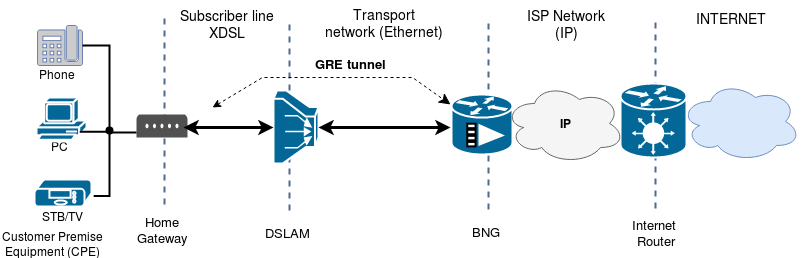
\includegraphics[width=0.8\linewidth]{figures/bng_architect.png}
 	\caption{Access Network Provider Model.}
 	\label{fig:arch}
\end{figure}
The network operator provides connectivity, authentication, applications and service network  policies to his users, therefore, these procedures involve the premise of session establishment using access communication protocols which are managed in the BNG, the most common protocols to establish session are:
\begin{itemize}
\item The PPP over Ethernet (PPPoE): Use the point-to-point (PPP) protocol.
\item The IP over Ethernet (IPoE): Use IP protocol that runs between CPE and BNG.
\item Generic Routing Encapsulation (GRE V2), encapsulation protocol brings virtual  Point-to-Point connections through IP network.
\end{itemize}
In our implementation, the packet sent or received by the HW are encapsulated with GRE headers, creating a point-to-point link with the BNG, but is just one of the options for packets encapsulation. \\
Since the BNG centralizes all the functions simplify the management functions like:
\begin{itemize}
\item Session management and header cap/decapsulation.
\item Interface to Authorization, Authentication and accounting services.
\item ARP proxy to manage the requests from the network interface on the BNG side.
\item Network Address translation to route the packets towards the operator’s core Network.
\item Interface to assignment queues and line rate to subscribers.
\end{itemize}
On the other hand, all these tasks make the structure of network rigid and become difficult to support the protocols and architectures in the current ISP.  In \cite{Rethinking} we found some similar approach to virtualize a Broadband Remote Access Server (BRAS) based on Click OS, a tiny Xen virtual machine designed specifically for network processing it can achieve line rate of 10Gbps and it composes of netmap and VALE as the packet I/O framework.
Our architecture approach goes with the same trend of network function virtualization using Macsad framework that compiles P4 code to bring more flexibility to the data plane and adding support for Hardware Abstraction Layer (HAL).\\
In the next session, we will describe our architecture design to be rapidly reconfigured using a “programming protocol-independent packet processors” (P4) and MACSAD to generate the datapath Logic codes.


% %%%%%%%%%%%%%%%%%%%%% subSection 2 P4 %%%%%%%%%%%%%%%%%%%%%%%%%%%%%%%%%%%
\subsection{Programming Protocol-Independent Packet Processors (P4)}
\begin{figure}[!h]
	\centering
	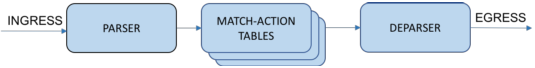
\includegraphics[width=0.7\linewidth]{figures/p4_dp.png}
	\caption{P4 Abstract Forwarding Model. Source: Adapted from \cite{P4}.}
	\label{fig:p4_dp}
\end{figure}
P4 is a high-level language for programming protocol-independent packet processors that define how the pipeline of a network forwarding device should process the packets using the abstract forwarding model (See figure \ref{fig:p4_dp}). P4 define the header structures and use the parser to extracts the header fields. The pipeline is defined through a series of match-action tables, which execute one or more actions like packet forwarding, drop and so on.  This tables can be changed and accessed at "runtime" through a controller software to add, remove and modify table entries and finally, de-parser writes the header fields back before sending the packets to the output port. The three main advantages of P4 are:

\begin{enumerate}
\item Reconfigurability in the field: Programmers should be able to change the way how the switch process the packets once that was deployed. 
\item Protocol independence: Capability to deploy any protocol in a switch.  
\item Target independence: To describe packet-processing functionality independent of the hardware where it has been deployed \cite{P4}.
\end{enumerate}

% %%%%%%%%%%%%%%%%%%%%% subSection 2 MACSAD %%%%%%%%%%%%%%%%%%%%%%%%%%%%%%
\subsection{Multi-Architecture Compiler System for Abstract Dataplanes (MACSAD)} 
\label{sec:Macsad}
This tool brings an environment to compile and deploy switch for L2/L3 applications automatically generating the datapath code for heterogeneous targets over 10Gbps network interfaces setup \cite{Patra}.\\
The MACSAD architecture is designed around the following three modules: (See the figure 2a) \\ \\
\begin{figure*}[!ht]
	\centering
	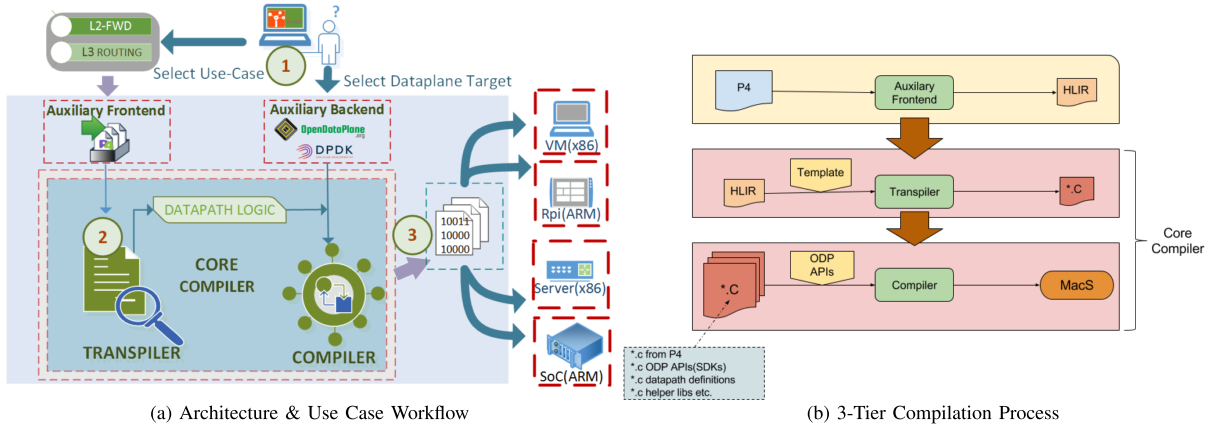
\includegraphics[width=0.85\linewidth]{figures/macsad_arch.png}
	\caption{Macsad architecture. Source:\cite{Patra}}
	\label{fig:mac_arch}
\end{figure*}

\textbf{- Auxiliary Frontend:} The P4 code is the MACSAD input that will be converted to an IR representation using the  p4-hlir framework that supports different Domain Specific Language (DSL) to generate a High-Level Intermediate Representation (HLIR) to be used in the Macsad core compiler.\\
\textbf{- Auxiliary Backend:} this module provides a common SDK for the Compiler incorporating the ODP APIs 
%  \cite{odp} 
 auto-generating support for different platforms with ODP supporting various control protocols like Switch Abstraction Interface (SAI), OpenFlow (OF), and other useful events for buffer like queueing, scheduling, etc.\\
\textbf{- Core Compiler:} Composed of a Transpiler and a Compiler submodule (see the figure \ref{fig:mac_arch}b), transforms the IR generated by the frontend into the target imaged in association with the auxiliary backend.\\
The transpiler takes the HLIR input and auto-generates the Datapath Logic codes. Some critical decision is taken in this sub-module like to optimize the ’Dead Code Elimination’ by identifying reachability in a graph, decides the type of look-up mechanism to be used, and size and type of tables to be created by. 
The Macsad compiler creates a set of libraries in 'C' codes for the desired target (x86, x86+DPDK, ARM-SoC).\\
The BNG P4 code will be added to the system as an input to create the BNG router. Also, Macsad tool brings the generation of high-level ODP APIs to deliver platform abstraction with high performance and hardware-acceleration options.



\subsection{Open Data Plane (ODP)}
Open Data Plane project provides an application programming environment for data plane applications with high performance and portable across a lot of HW platform.
The aim of ODP is separate application design from the functional implementation of that design, this because historically it requires that data plane application must be redesigned on changes in network speed and capacity because the applications need to be very integrated with specialized hardware to achieve acceptable performance levels.
ODP relies on the Linux kernel itself; it defines some ODP API set to rapid porting ODP application to any platform (See Figure \ref{fig:sys_arch}), it can define functions and limits like a number of queues or used cores processor.\\
% %%% -----------
\begin{figure*}[!ht]
	\centering
	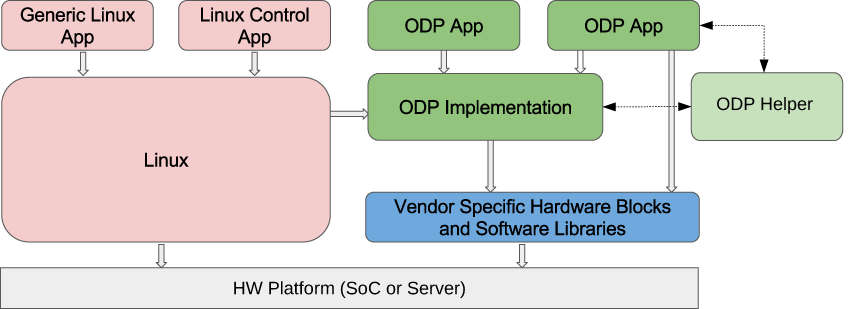
\includegraphics[width=0.6\linewidth]
     {figures/odp-overview.png}
% 	\caption{ODP system architecture. Source:\cite{opd_spec}}
 	\caption{ODP system architecture. Source:....}
	\label{fig:sys_arch}
\end{figure*}
ODP applications can run in parallel with full Linux user processes that implement control and management functions since that these typically do not have critical performance and latency requirements. In that sent, this tool calls the Software Development Kit (SDK) and optimize the features and functionalities for the particular hardware platform (SoC or Server).
The ODP APIs is written in the C programing language and are optimized to control related SoC resources such as:
\begin{itemize}
\item CPUs (or hardware threads) 
\item Main memory
\item Huge page mappings (how many, what sizes) 
\item Physical and virtual ports/interfaces 
\item Packet classification rules 
\item Scheduler (core groups, algorithms, ordering) 
\item Hardware queues 
\item Output traffic management 
\item hardware Quality of Service (QoS) support. 

\end{itemize}



\chapter{Related works}
\label{cap:cap03}

The work in \cite{Rethinking} presents an implementation of a BRAS/BNG using an alternative framework called Click. It comes with hundred of simple elements. Moreover, it uses tiny virtual machines that can boot quickly and have a small memory footprint,  it lends itself to a good platform for NFV, and the results reported focus on the overall performance of a number of session establishment rate and memory consumption when establishing sessions instead of the impact of design decisions on performance.\\

The work in \cite{Masutani} describes a BNG implementation but focuses on a vendor-neutral architecture suitable for standardization. They present the requirements and a basic design of
a flexible and elastic network service infrastructure with NFV and SDN/OpenFlow. Our work differs in that adds other features such as multi-architecture target using MACSAD tool and P4 language in order to add more flexibility and application performance.\\

The work in \cite{Nemeth} exposes the performance implications related bandwidth constraints, Virtual Network Function (VNF) placement during service deployment.  They illustrate this with a “proof of concept” implementation of a Broadband Remote Access Service (BRAS)/Border Network Gateway (BNG) using Data Plane Development Kit (DPDK) \cite{dpdk}. The performance focuses on the QoS function, the most resource demanding function of their prototype, and the impact of core layout and memory usage on performance.\\


In order to turn more flexible \cite{Pongracz} describes the implementation of a router using DPDK. He reported forwarding rates between 5.26 Gbps and 9.6 Gbps for packet sizes of 64B and 512B, respectively, with one OpenFlow 1.3 implementation as the primary model of SDN data plane. Our routing functions are substantially similar to theirs, and both implementations use DPDK framework to add functionalities to the network device.\\


The work in \cite{Hwang} describes the design of software router, with some network functionalities such as Layer 3 forwarding, a firewall that resides in distinct VMs on the NetVM platform obtaining throughputs up to 10 Gbps. Rather of running into hardware limitations such as NIC, their implementation is limited by the available processing capacity.\\

The work in \cite{Woesner} shows a BRAS / BNG demo scenario to migrate PPPoE / PPP-based Internet access to a plain IPoE network functionalities and develop BNG and BRAS prototypes into an orchestration framework triggered by an SDN and NFV control. Unlike our proposed work their implementation doesn't have results of the implementation as such as worst and best cases of throughput neither functionalities validation, application performance and memory usage.\\

In \cite{Rahimi} they evaluated the impact of certain parameters and settings in a software switch called Lagopus on which were implemented L2 and L3 network layer functionalities using Intel’s Data Plane Development Kit (DPDK) and OpenFlow.\\
This work focused on application performance using a software called “pktgen” achieving  maximum throughput of 9.8 Gbps when the packet size was 1500B and 100K OpenFlow entry tables in other hand they studied packet drop rates and presented the impact of parallelization on switch performance, which includes both packet forwarding rate and packet drop rate, at high loads in a configuration with high link rates it demonstrates the importance of receive-thread packet classification for load balancing and to send delay-sensitive flows to a different worker thread from high-throughput flows.

Main related projects around BNG software switch implementations and data plane support mentioned above are summarized in Table \ref{table:related_w}:

\begin{table}[H]
	\begin{tabular}{ >{\arraybackslash}m{20cm}}
		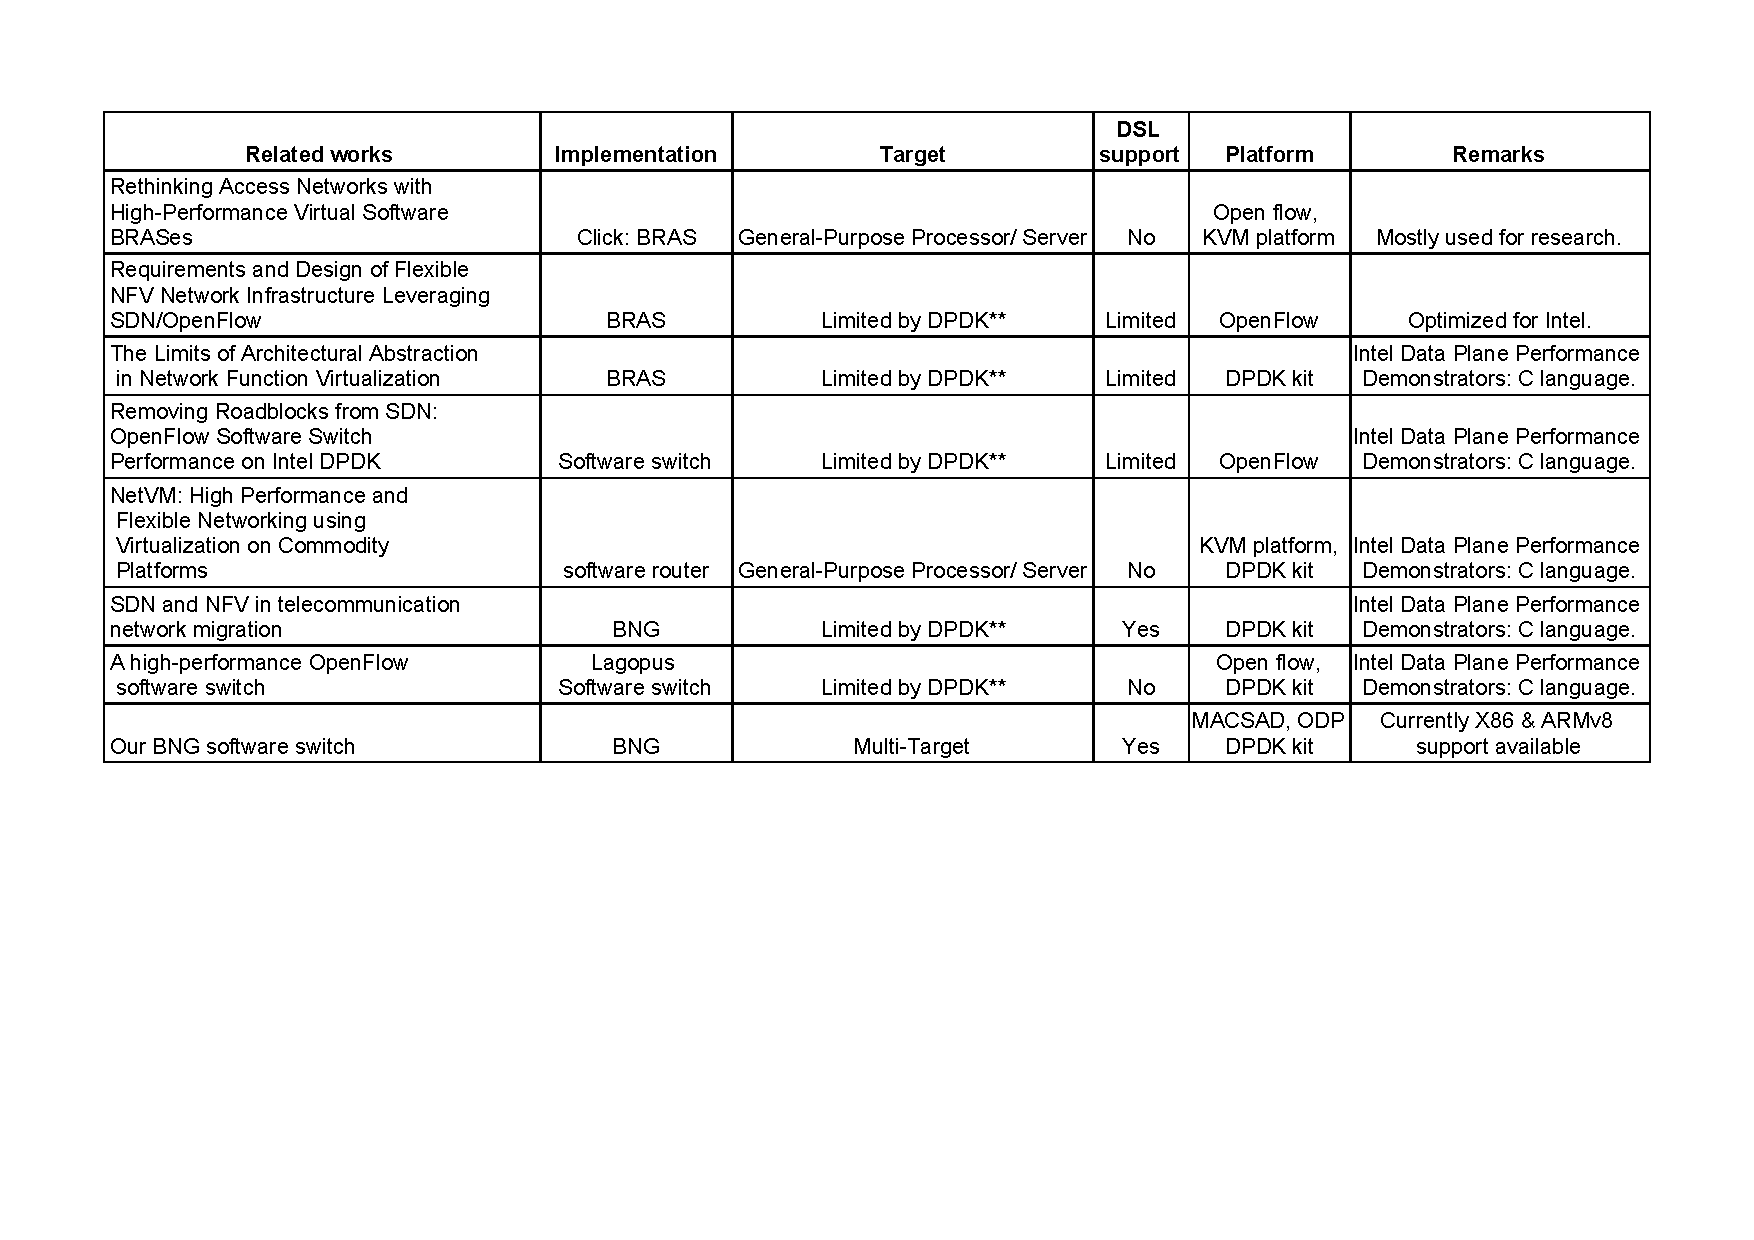
\includegraphics[width=18cm]{figures/related_w.pdf} 
	\end{tabular}
	\caption{Feature comparison list of different Switch software implementations.}
	\label{table:related_w}
\end{table}

\chapter{Development}
\label{cap:cap04}

This chapter covers the software switch development. In section \ref{softfeatures}, we give details about the implementation of the most important OpenFlow 1.3 features, in section \ref{OpenSourceDev}, we describe the open source model adopted for the software switch development. 

\section{Software switch implementation}
\label{softfeatures}

Implementation of an OpenFlow switch depends on the platform for which it is designed. OpenFlow hardware implementation on traditional Application Specific Integrated Circuit (ASIC) chips usually suffer from limitations, like small capacity in the total number of flows and not real support for multiple tables. Unlike hardware, software implementations offer greater flexibility in the implementation of OpenFlow features. In environments where high throughput is not the biggest concern, software switches running on commodity servers can be a low cost replacement option for traditional network switches.

The OpenFlow specification describes OpenFlow switches pipeline and the required and optional building blocks. It does not gives low level details about how these components should be implemented. As long as it works how the specification dictates, switch designers are free to use any data structures and algorithms in order to implement OpenFlow. When defining implementation details, we explored the software implementation freedom to meet the requisites defined on section \ref{sec:sec02}. At the same time, we came up with innovative design decisions towards future extensions of the OpenFlow match field support.  

In this section we discuss how we implemented the OpenFlow 1.3 software switch adding several changes to the base switch - using C \footnote{In this chapter there will be two common words: struct and structure. While struct is a C language keyword and structure is a more generic word for a collection of data variables, both will be used to denote a C struct.}, the switch native programming language, and C++ - in order to support all features and keep it as simple as possible. The next subsections describe this new functionalities in the context of the architecture of the software switch presented in chapter \ref{cap:cap03}.

\subsection{Oflib}
\label{sec:sec41}

The software switch architecture Marshaling/Unmarshaling library, presented in section \ref{(un)pack}, is called Oflib. Although already present in the software switch base code, the library underwent several modifications in old messages and grew with the addition of OpenFlow 1.3 messages.

Every OpenFlow message represented by the Oflib has a common header. This header struct contains only one member, which is the message type information. Using the same initial struct for every message struct allows the implementation of two general functions that abstract marshaling and unmarshaling. In the Listing \ref{msgpackunpack}, we show the definition of these functions. Marshaling, also known as packing, is done by \textit{ofl_msg_pack}. By passing a pointer to the struct \textit{ofl_msg_header} for the function, we can check the message type and apply the message respective marshaling function. Unmarshaling, also known as unpacking, is performed by \textit{ofl_msg_unpack}. In this function, the first bytes of the OpenFlow messages, the \textit{buf} parameter, reveal their types. With this information the function calls the proper function to convert the message for the Oflib format.  
\begin{lstlisting}[caption={Oflib: message pack and unpack base functions}, label=msgpackunpack,]
int ofl_msg_pack(struct ofl_msg_header *msg, uint32_t xid, uint8_t **buf, size_t *buf_len, struct ofl_exp *exp);

ofl_err ofl_msg_unpack(uint8_t *buf, size_t buf_len, struct ofl_msg_header **msg, uint32_t *xid, struct ofl_exp *exp);
\end{lstlisting}

Another Oflib task, discussed in the section \ref{(un)pack}, is message error handling. It checks for bad requests from the controller, for example messages with unknown types and wrong sizes are performed by every unpacking function. In case of error, the function returns the OpenFlow error code for the Datapath, which creates an error message and sends it for the controller, through the Communication Channel.

Addition of new OpenFlow messages in the Oflib is a trivial task. Firstly, the developer needs to define a C struct, with \textit{struct ofl_msg_header} as the first member. Then, write a pack and unpack function. Finally, add the new message type for \textit{ofl_msg_pack} and \textit{ofl_msg_unpack}. Listing \ref{rolerequest} illustrates the OpenFlow 1.3 \textit{Role Request}, implemented during our work. 
\pagebreak
\begin{lstlisting}[caption={Oflib message Role request struct and function definition}, label=rolerequest,]
struct ofl_msg_role_request {
	struct ofl_msg_header header; /* Type OFPT_ROLE_REQUEST/OFPT_ROLE_REPLY. */
	uint32_t role;                /* One of OFPCR_ROLE_*. */
	uint64_t generation_id;       /* Master Election Generation Id */
};

static ofl_err
ofl_msg_unpack_role_request(struct ofp_header *src, size_t *len, struct ofl_msg_header **msg)

static int
ofl_msg_pack_role_request(struct ofl_msg_role_request *msg, uint8_t **buf, size_t *buf_len)
};
\end{lstlisting}

Additionally, the Oflib also has printing functions. This is helpful for logging and debugging in the software switch.      

\subsection{OpenFlow Extended Match}
\label{sec:sec42}

When compared to OpenFlow 1.1, in the number of supported match fields, the version 1.3 of the OpenFlow protocol supports nearly twice as much fields as the former version. This growth was only possible due to changes in the match structure specification. A match structure from OpenFlow 1.1 was a fixed number of fields, carrying 88 bits of information in every message carrying a new flow. Match fields not set in the message were sent, adding unnecessary space overhead.   
In order to keep the protocol evolution and to support more fields, the OpenFlow Extended Match (OXM) was introduced by the OpenFlow 1.2 specification. The OXM format is Type-Lenght-Value (TLV) based and replaces the old fixed match structure. A less restricted definition of the match struct adds more flexibility for the insertion of new match fields. Figure \ref{fig:oxmfield} shows an example of how a field is defined by an OXM field and the TLV respective sizes in bits. The Type of a match field is formed by the OXM Class and OXM Field. An OXM class represents a vendor number, where 0x8000 is the basic class for the specification of the match fields. OXM Field defines the match field. In the example, the field number 15 represents the UDP protocol in OpenFlow. The last bit of the Type is left for the Has Mask field, which indicates if the match is masked or not. Finally, the Length field is the value size.
\\
\begin{figure}[H]
\centering
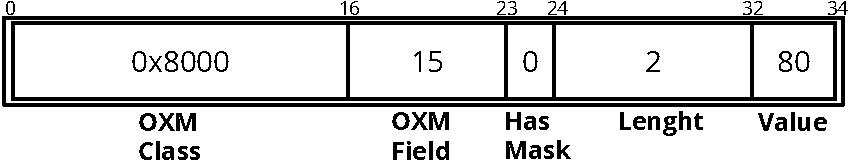
\includegraphics[height=3cm,width=\textwidth,keepaspectratio]{eps/OXMfieldexample.pdf}
\caption{OXM field example}
\label{fig:oxmfield}
\end{figure}

Some challenges arise with the OXM introduction. Whereas extension of match support for messages is solved, there is nothing concerning the packet parsing in the Datapath. The next subsections discuss how our implementation deals with protocol fields extensibility in the software switch. 

    \subsubsection{Packet Parser}
    \label{pktparser}

    Each new protocol added for the OpenFlow specification demands the addition of an specific code to extract the new fields. Distinct protocols may have singular and complex parsing methods. For instance, variable fields such as IP options can require cumbersome deep packet inspection. For this reason, the Packet Parser implementation needs to be flexible and easy to extend. Also, the idea of simple insertion of new match fields meets the ease of extension requisite.    
    
    As a means to achieve a Packet Parser implementation featuring the mentioned characteristics, we have come up with a design which uses a packet description language to assist the parsing. Figure \ref{fig:netbee} shows the Packet Parser model implemented on the switch Datapath. Each module is described as follows:
    
    \begin{figure}[h]
    \centering
    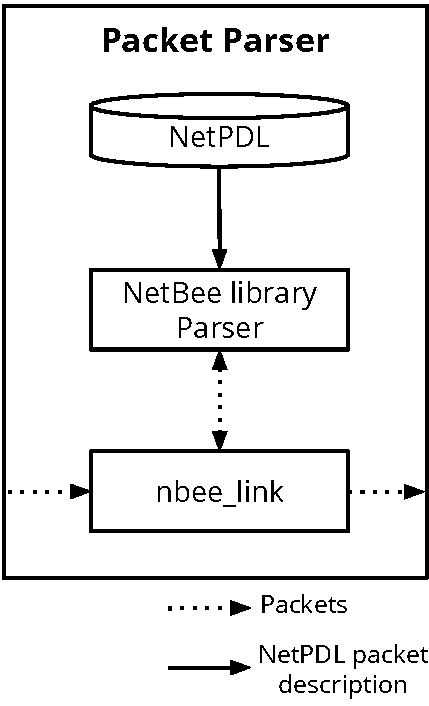
\includegraphics[height=9cm,width=\textwidth,keepaspectratio]{eps/PacketParserEngine.pdf}
    \caption{Packet Parser components}
    \label{fig:netbee}
    \end{figure}
    
    \begin{itemize}
    \item \textbf{NetPDL}. The Network Protocol Description Language (NetPDL)\cite{Risso:2006:NEX:1141112.1141119} is the packet description language. It is a XML-based language and has a large number of protocols and specified encapsulations. In addition, the simple language definition allows easy and fast addition of non available protocol description. An example of how the UDP protocol is described using NetPDL can be foung in the Annex \ref{annex:NetPDLdesc}. In the Figure \ref{fig:netbee} the NetPDL module feeds the parsing library with the description of the OpenFlow 1.3 supported match fields.
    
    \item \textbf{NetBee library Parser}. Netbee is as library for packet processing \cite{nbee}. It is composed by several modules for different types of network application, such as packet filtering and sniffing. For our Packet Parser implementation, we use the Netbee library decoding objects. These objects come from a C++ set of classes and methods that ease packet decoding. To accomplish this, firstly Netbee loads the NetPDL protocols specification into the machine Random Access memory (RAM) and on a packet. Then, received packets are decoded according to the NetPDL description and the extracted information is stored in a protocol tree. Finally, packet field values can be retrieved from the tree using specific methods of the library. 
    
    \item \textbf{nbee_link}. This module is where packets are converted in the flow match structure. Arriving packets are sent for the Netbee library for decoding. From the protocols tree generated by Netbee, the nbee_link module   
extracts the field values and builds the packet match structure that will be sent to the Flow Table look up. The code to extract a protocol is shown by Listing \ref{nbeeparsing}. Using the Netbee method \textit{GetPDMLField}, we get the three ethernet protocol supported fields in OpenFlow 1.3. The second argument of \textit{GetPDMLField} reflects the field name defined in the NetPDL specification. The function \textit{nblink_extract_proto_fields} receives the extracted field value and type and inserts this into the match structure. Another important piece of code is present in the third line. For possible further processing, for instance, the application of a \textit{set field} action, a reference to the protocol position needs to be stored. 
    \pagebreak
    \begin{lstlisting}[caption={Ethernet parsing in the nbee_link module}, label=nbeeparsing,]
    if (protocol_Name.compare("ethernet") == 0 && pkt_proto->eth == NULL)
    {
        pkt_proto->eth = (struct eth_header *) ( (uint8_t*) pktin->data + proto->Position);
        PDMLReader->GetPDMLField(proto->Name, (char*) "dst", proto->FirstField, &field);
        nblink_extract_proto_fields(pktin, field, pktout, OXM_OF_ETH_DST);
        PDMLReader->GetPDMLField(proto->Name, (char*) "src", proto->FirstField, &field);
        nblink_extract_proto_fields(pktin, field, pktout, OXM_OF_ETH_SRC);
        PDMLReader->GetPDMLField(proto->Name, (char*) "type", proto->FirstField, &field);
        nblink_extract_proto_fields(pktin, field, pktout, OXM_OF_ETH_TYPE);
    }
    \end{lstlisting}      
    
    \end{itemize}
    
    An example of how helpful is a flexible design for the Packer Parser is on the support for IPv6 Extension Headers (EH) \cite{rfc2460}. EHs parsing execution is not a trivial task, as there are different types and formats. What is more, IPv6 packets may present complex combinations of headers. In OpenFlow 1.3 support for IPv6 EHs is not based on values, but on a special bitmap that matches in the presence of EHs. Besides, a bit field matches an IPv6 packet only if their EHs are in the recommended order. All of these details would result in a large ammount of code to parse EHs correctly. However, this is done in few lines due to our extensible implementation and the NetPDL language.    
    \subsubsection{Flow Match Prerequisites}
    
    Another change brought by OXMs is the introduction of flow match fields prerequisites. In order to obtain flow match consistency, some match fields require the presence of other fields. For example, matching any ARP protocol field requires the ethertype field having the correct value for an ARP packet. Thereby, inconsistent flows are denied by the Flow Table.  
      
    To map OXM fields prerequisites, a file \footnote{This file was inpired by the old way that OVS handled the Nicira Extended Match (NXM) format. NXM is the format that gave origin to OXM.}, with several C Preprocessor macros, was created. The macros map each field with their respective network layer 2, layer 3 or upper level requisite. In addition there is a field that tells if a field is maskable or not. Listing \ref{oxmrequisite} shows prerequisites and fields macros definition. Also, it gives an example of a field created by the \textit{DEFINE_FIELD} macro. 
\\
\begin{lstlisting}[caption={Ethernet parsing in the nbee_link module}, label=oxmrequisite,]

#define OXM_DL_NONE   (0, 0)
#define OXM_DL_ARP    (ETH_TYPE_ARP, 0)
#define OXM_DL_PBB    (ETH_TYPE_PBB,0)
#define OXM_DL_IP     (ETH_TYPE_IP, 0)
#define OXM_DL_MPLS   (ETH_TYPE_MPLS, ETH_TYPE_MPLS_MCAST)
#define OXM_DL_IPV6   (ETH_TYPE_IPV6, 0)
#define OXM_DL_IP_ANY (ETH_TYPE_IP, ETH_TYPE_IPV6)

#define DEFINE_FIELD_M(HEADER,  DL_TYPES, NW_PROTO, MASKABLE)  \
    DEFINE_FIELD(HEADER,  DL_TYPES, NW_PROTO, MASKABLE)        \
    DEFINE_FIELD(HEADER##_W, DL_TYPES, NW_PROTO, true)

DEFINE_FIELD    (OF_TCP_SRC,        OXM_DL_IP_ANY,   IPPROTO_TCP,    false)

\end{lstlisting}   

    OXMs matches definitions are loaded by the Oflib, and used in the function \textit{oxm_pull_match}, which is called during the match unpack. Among the tests performed to detect invalid OXM fields are: bad prerequisite, duplicate fields, wrongly masked and nonexistent field.  

    \subsubsection{Flow Matching}
    
    In the pursuit for the best way to perform flow matching inside the Flow Table, developers might want to try different algorithms and data structures. For this reason, the switch implements a flexible and easy interface to change the way packets are matched. 
    
    Match fields are part of the software switch \textit{flow_entry} struct. Instead of defining a fixed match as one of the \textit{flow_entry} member, a pointer to Oflib \textit{struct ofl_match_header} is left as a reference for the entry match fields. Therefore, if a developer wants to experiment his own match structure, there is only the need to make it start with an \textit{ ofl_match_header}.    

    This work presents a default flow matching using the Oflib match structure called \textit{ofl_match}. Besides the match header, the struct includes a Hash Map structure to store OXM TLVs. Each OXM entry in the Hash Map has an  exclusive key, created by the combination of the field Type and Length information. Storing only flow specified fields saves memory space, at a small cost of the pointers created to mantain the data structure. Another advantage in the Hash Map use in the match structure is the constant access time for the OXMs. Fast element access is very important for two of the most common operations:
    
    \begin{itemize}
    \item \textbf{Check packet matching}. Packet fields are extracted and matched against the flows. Matching is performed by look ups of the packet fields in the Hash Map.        
    
    \item \textbf{Check flow collision}. Flows collide when a new flow is installed and the Flow Table contains a flow with the same match fields and priority. In this case the old one is replaced by the new one. The Hash Map allows a direct comparison of fields.
    \end{itemize}

    Another detail about flow matching in the software switch is about the linear behavior of Flow Table look up. The Flow Table stores flows in a list ordered by priority. When a packet is sent to the flow match it loops through the flow list until it finds a matching rule or it reaches its end. This is the most simple approach for the flow match and was chosen for its simplicity. Developers who might want to modify the behaviour of Flow Table look up just need to add their own code for the function \textit{flow_table_lookup}.
         
    \subsubsection{Extensible context expression in ’packet-in’}
    
    Former \textit{packet-in} message contained little information about the packet parsed in the Datapath. The only match field present was the switch input port. In order to get the other packet fields, a controller needs to parse the packet header, included in the end of \textit{packet-in}. This causes an unnecessary parsing repetition in the control plane. With the OXM introduction, OpenFlow 1.3 solves this problem sending the extracted packet fields in the form of OXMs, making it easier for the control plane to retrieve the packet fields.  
    
    While an standard switch implementation requires only context information, which are input port, metadata and tunnel_id, our implementation follows the option to add all parsed fields in a \textit{packet-in} message.    

\subsection{Set Field action}
\label{sec:sec43}    

Support for rewriting packet fields exists since the first OpenFlow version. However, it was limited to a small set of fields. In OpenFlow 1.3, with the OXM introduction, a \textit{flow mod} message can carry a  \textit{set field} action with any of the OXMs defined by the specification. It is up for the switch designers to decide which fields are allowed for overwrite.   

Implementation of \textit{set field} is slightly intricate, as the consistence is achieved through the match fields. For instance, a flow with a \textit{set field} action to rewrite the IP source address needs to present in the match fields the same ethertype - 0x800 in hexadecimal - of the IP protocol. The way the pack and unpack of match fields and actions is performed by different functions needs to be checked in the Datapath. When handling a new \textit{flow mod} message, the Flow Table calls the function \textit{dp_actions_check_set_field_req}. This function uses an Oflib function to check if the prerequisites are ok and validates the action.

Another frequent task caused by rewriting fields is protocol CheckSum recalculation. Fields like the IP source and destination, in the case of change, require recalculation of IP and TCP CheckSum values. Fortunately these protocols' CheckSum calculation is very simple \cite{rfc1071}. This is not the case for the SCTP protocol \cite{rfc3309}. SCTP CheckSum is calculated using a Cyclic Redundancy Check (CRC). In order to recalculate the SCTP CheckSum value we used a Python program named pycrc \footnote{pycrc v0.8.2, Available at http://www.tty1.net/pycrc/}. The program takes as input the CRC polynomial and generates all the functions necessary for the calculations. Listings \ref{set_field} shows the code to rewrite the SCTP destination port. In the packet field rewriting we attribute a pointer to the protocol struct representation and to the packet position obtained by the Packet Parser. Doing so, we can easily change the current value of the action value.
\\
\begin{lstlisting}[caption={Ethernet parsing in the nbee_link module}, label=set_field,]
case OXM_OF_SCTP_DST:{
                crc_t crc;
                struct sctp_header *sctp = pkt->handle_std->proto->sctp;                
                size_t len = ((uint8_t*) ofpbuf_tail(pkt->handle_std->pkt->buffer)) - (uint8_t *) sctp;
                uint16_t v = htons(*(uint16_t*) act->field->value);
                sctp->sctp_csum = 0;
                memcpy(&sctp->sctp_dst, &v, OXM_LENGTH(act->field->header));
                crc = crc_init();
                crc = crc_update(crc, (unsigned char*)sctp, len);                            
                crc = crc_finalize(crc);
                sctp->sctp_csum = crc;
                break;        
            }
\end{lstlisting}  

\subsection{Per-flow Metering}

    The Meter Table implementation follows the architectural details and responsibilities of the element described on section \ref{sec:MeterTable}.
Firstly we defined a structure for the Meter Table. The main components are the table features, such as the max number of entries and supported band types, and a Hash Map of meter entries. Other members include a reference pointer to the Datapath, allowing a Meter Table to call the function to send OpenFlow messages; and two counters: one for the number of meter entries and another one for the quantity of bands. Secondly, we implemented a set of functions: initialization and destruction of the Meter Table; \textit{meter mod} and \textit{meter features} messages handlers; find and apply a meter entry.

    Structures of meter entries are composed of a configuration - which contains information about the meter id and meter bands - and a struct for recording statistics. In addition, the meter entry has pointers to the Datapath and the Meter Table, similar to what is done in the Meter Table struct. Finally, it has a list of flow references. If the meter entry is deleted, all flows sending packets to the meter entry are deleted. 

    Meter entry bands are chosen accordingly to a configured rate - in Kilo packets (Kpps) per second or Kilobits per second (Kbps). Thus, it is necessary to measure the flow matched packets in function of one of the specified unities. The first idea to implement rate measuring scheme considered the use of matched flow counters, divided by the number of matched bytes by some time interval. Although easy to implement, this approach proved itself inaccurate after some attempts to limit the bandwidth between two hosts connected to the switch.  
    
    After a better analysis of the task and some literature research, we found and implemented a simple and efficient algorithm used for rate policy: the Token Bucket \cite{Tanenbaum:2002:CN:572404}. Figure \ref{fig:tokenbucket} illustrates how the Token Bucket works within a meter band. Simply put, each meter band has a bucket attached to it. At every second the bucket is refilled with a number of tokens equal to the meter rate. When a packet is sent to the Meter Table, it goes through each band's bucket belonging to the meter entry. Inside the bucket, packets consume a number of tokens equal to their size. If there are enough tokens, the OpenFlow pipeline continues processing the packet, otherwise, the meter band is chosen and executed.               

    \begin{figure}[h]
    \centering
    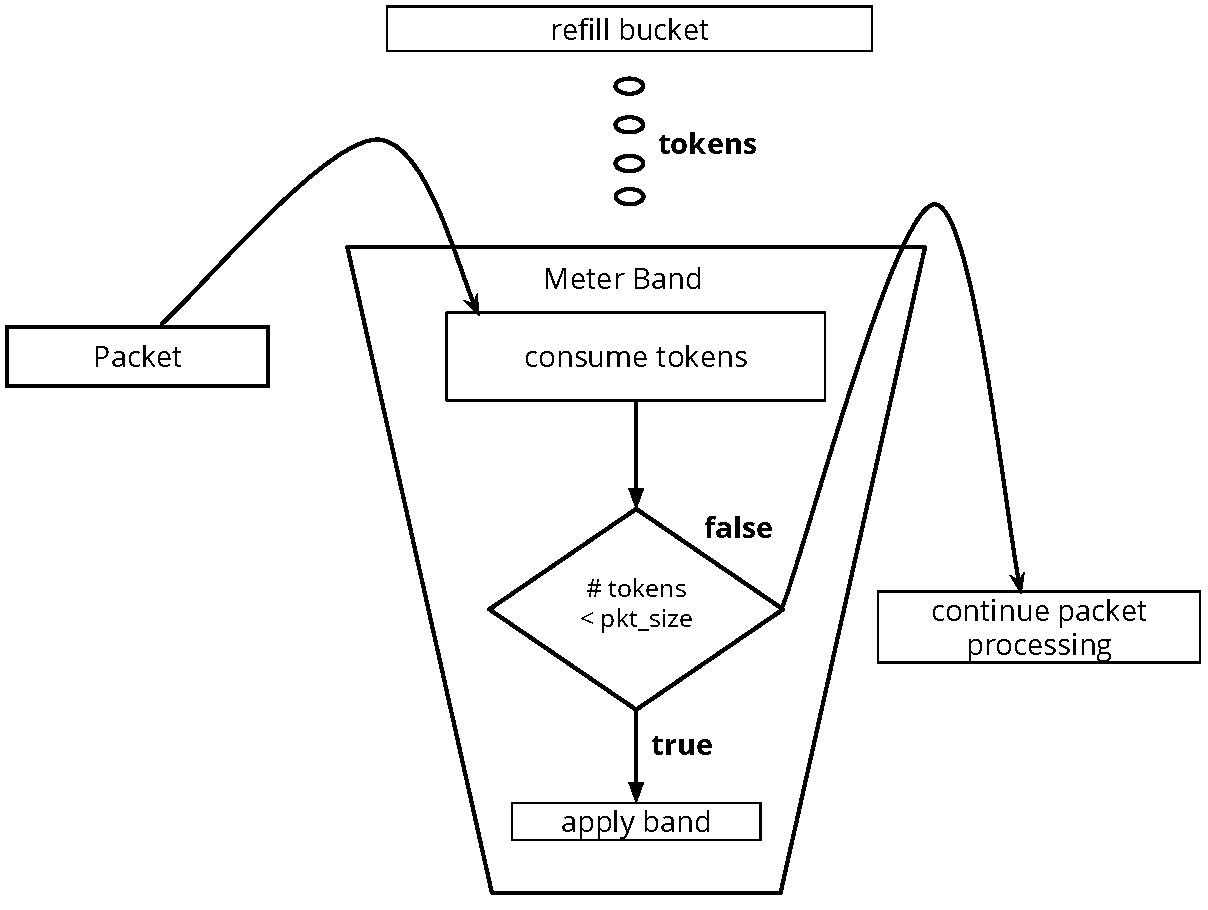
\includegraphics[height=9cm,width=\textwidth,keepaspectratio]{eps/TokenBucket.pdf}
    \caption{Token Bucket Algorithm illustration inside the meter band}
    \label{fig:tokenbucket}
    \end{figure}

\label{sec:sec44}

\subsection{Connection Features}
\label{sec:sec45}

    Network control protocols must be designed with scalability and high availability in mind. Node failures and high traffic loads may cause frustration for early adopters of new technologies, as these two important points are not usually considered by initial versions. Previous OpenFlow versions fall into this category of protocols, often criticized by the lack of mechanisms to handle control plane issues. 
    
    More recent OpenFlow versions try to address control plane scalability and high availability with the addition of new features for OpenFlow connections. Auxiliary connections allow higher scalability for message exchanging, while controller roles try to enable fast failover for OpenFlow controllers. Event filtering, in turn, may be seen as a mechanism that sum up on these two topics. In the next subsections we will see a more detailed description of each feature and how they have been implemented in our software switch.
    
    \subsubsection{Auxiliary Connections}
    
    Auxiliary connections allow a controller to create more than one Communication Channel with a single switch. These connections add the possibility to exploit message parallelism and create a channel for specific types of messages. For instance, a controller can use one connection only for \textit{packet-in} messages. 
    
    As a proof-of-concept we have implemented basic support for auxiliary connections. In our implementation, there is support for only one additional channel and it only carries \textit{packet-in} messages. The following items show steps added in the switch code to handle auxiliary connection.
    
    \begin{itemize}
    \item The software switch sends OpenFlow messages for the Communication Channel, encapsulated into a struct called \textit{ofbuf}. The struct is a buffer that holds information such as the pointer for the first allocated byte and the size of bytes in use. In order to identify which connection is being used to receive or send the message, we have added a new member called \textit{conn_id}. The possible values for \textit{conn_id} are MAIN_CONNECTION and PTIN_CONNECTION.  
    
    \item A new connection listener was added to the Datapath. If an auxiliary connection is specified when running the datapath, the auxiliary listener is opened after the main connection listener.
    
    \item When the Datapath talks to remotes, it searches for the auxiliary connection. If the connection exists, it processes messages received by the connection.
    
    \item On sending OpenFlow messages, the switch by default maps to the MAIN_CONNECTION. If the message is a reply from  a sent message of a sender connection, the connection id is set to the same id used by the sender. In the last case, if the message type is a \textit{packet-in}, the switch uses PTIN_CONNECTION for the connection id. 
    
    \end{itemize}
    
    The start of an auxiliary connection from one controller is disabled by default in our software switch standard program execution. To enable auxiliary connections a user should specify the \textit{multiconn} option in the command line option.   

    \subsubsection{Controller Role}

    Controller Role is a mechanism to permit connection of multiple controllers with different duties. One of the possible use cases of roles is for fast failover, in which when the main controller goes down, a backup controller assumes the switch command. There are three possible roles for controllers: Master, Slave and Equal. A master controller has permissions to send and receive any type of OpenFlow messages. Slaves have very strict default permissions, allowed only to receive a specific set of messages. The last role, Equal, is the default role when a controller connects to the switch and the other controllers connected do not have a defined role.
    
    Role election is totally driven by the control plane, though some additional code is required for the switch. In order to implement controller role support in our software switch we first filtered asynchronous messages received by Slave controllers. Then we restricted slaves to send only read state messages, for example, \textit{flow stats} and \textit{table stats}. The last insertion is the algorithm defined by the specification to handle the \textit{role request} generation_id. Messages with a generation id smaller than previous generation ids seen by the switch are discarded. Listing \ref{rolegenid} presents the function that implements the algorithm.
\pagebreak
\begin{lstlisting}[caption={Ethernet parsing in the nbee_link module}, label=rolegenid,]
static ofl_err
dp_check_generation_id(struct datapath *dp, uint64_t new_gen_id){

    if(dp->generation_id >= 0  && ((uint64_t)(new_gen_id - dp->generation_id) < 0) )
        return ofl_error(OFPET_ROLE_REQUEST_FAILED, OFPRRFC_STALE);
    else dp->generation_id = new_gen_id;
    return 0;
}
\end{lstlisting} 
    \subsubsection{Event Filtering}

    Event Filtering enables controllers to filter undesired asynchronous messages, sent by the switch. Filtering of asynchronous messages is possible for three types: \textit{port status}, \textit{packet-in} and \textit{flow removed}. In addition, a controller can also choose to not receive these message types for the generation reason. For example, a \textit{packet-in} can be generated by an action to output the packet for the controller. This feature, along with auxiliary connections, gives power for controllers to create exclusive message channels.
    
    Message filtering is handled by the Datapath. On a \textit{set async request}, the Datapath sets the controller remote channel with bitmap values sent in the message defined by the OpenFlow 1.3 specification, shown on Listing \ref{asyncmessage}. Each bit set in the bitmap represents a message type and a reason. For instance, a bit with value 4 in \textit{flow_removed_mask[0]}, determines if the controller will receive \textit{flow removed messages} with reason OFPRR_DELETE when the role is Master.  
    
    Filtering happens before the sending of an OpenFlow message. The Datapath function to send an OpenFlow buffer through the Communication Channel checks the remote configuration and the type of message to be sent. If it is one of the three asynchronous messages and the reason and the controller roles matches the remote filtering configuration, the message is dropped. 
    
\begin{lstlisting}[caption={Ethernet parsing in the nbee_link module}, label=asyncmessage,]    

/* Asynchronous message configuration. */
struct ofp_async_config {
    struct ofp_header header;
    /* OFPT_GET_ASYNC_REPLY or OFPT_SET_ASYNC. */
    uint32_t packet_in_mask[2];
    /* Bitmasks of OFPR_* values. */
    uint32_t port_status_mask[2]; /* Bitmasks of OFPPR_* values. */
    uint32_t flow_removed_mask[2];/* Bitmasks of OFPRR_* values. */
};
OFP_ASSERT(sizeof(struct ofp_async_config) == 32);

\end{lstlisting}






 
\chapter{Evaluation}
\label{cap:cap05}

In this chapter we evaluate our work in terms of the requisites presented on section \ref{sec:sec02}. The first section shows in numbers how many features are covered by the software switch. Subsequently, in the next section, we present the results of performance benchmarks tests. The last section of the chapter is a qualitative evaluation about the code's ease to change. We demonstrate the code portability, highlighting the port of the software switch to another processor architecture in a different operating system.      

The software switch evaluated version dates from the last commit pushed to GitHub. The box below shows the dates and last code changes description.

\begin{framed}

\begin{itemize}
\item \textbf{commit} cb740bd2565ac7e5d61ebe30ee75160a5452a033
\item   \textbf{Commit:}     Eder Leão Fernandes <ederleaofernandes@gmail.com> 
\item \textbf{CommitDate:} Mon Feb 23 18:42:49 2015 -0300 
\end{itemize}
     
    Add flags member to ofp_flow_stats.
    
    Fix missing flags field in the response of a flow stats request.
\end{framed}

\section{Feature Completeness}
\label{sec:FeatureComplete}
Evaluating the proper operation of the OpenFlow switch features is not a trivial task. This is caused by the multiple and rich configurations allowed by the specification. For example, testing all flow match fields combinations would require creation of a large number of flows and packets, making manual tests very time consuming. For this reason, automatic test frameworks, discussed on section \ref{sec:testemulation}, are the best options to test the switch functionality in order to evaluate feature completeness.    

OFTest and Ryu Certification are the two test frameworks used for the switch validation. As mentioned in chapter \ref{CodeMaintenance}, both are important tools for the software switch development. While Ryu certification has a strong focus on validation of the Datapath, OFTest offers a nice set of test cases for control and data plane message exchange. In the next sections we present a resume of the results obtained.  


\subsection{OFTest results}

Testing in OFTest is simple as it provides scripts in Python to run the switch and the test cases. Each test case starts a controller which connects with a running switch, executes the test instructions and checks the switch answers. 

Some messages from controller to switch, like a \textit{flow stats} request, and symmetric messages demand an answer from the switch. Thus, the main purpose of the framework usage with the software switch is for message handling validation. Although OFTest has capabilities to evaluate the pipeline processing - for instance, checking if a packet was correctly forwarded by a flow - we found in Ryu a more comprehensive test set for this task. 

Table \ref{tab:oftestbasic} shows test results for basic OpenFlow messages. The major type of messages of the test set are messages to query information about the state of manifold switch elements, such as \textit{GroupFeatureStats} and \textit{MeterStats}. Also, there are some configuration messages, like the \textit{PortConfigMod}. In all tests the switch returned the right answer for the control plane.


\begin{table}[h]
\centering
\caption{Basic OpenFlow messages}
\label{tab:oftestbasic}
\begin{tabular}{|l|l|l|l|l|}
\cline{1-2} \cline{4-5}
\multicolumn{1}{|c|}{\textbf{Message}} & \textbf{Result} &  & \textbf{Message}   & \textbf{Result} \\ \cline{1-2} \cline{4-5} 
AggregateStats                         & ok              &  & GroupFeaturesStats & ok              \\ \cline{1-2} \cline{4-5} 
AsyncConfigGet                         & ok              &  & GroupStats         & ok              \\ \cline{1-2} \cline{4-5} 
DescStats                              & ok              &  & MeterConfigStats   & ok              \\ \cline{1-2} \cline{4-5} 
Echo                                   & ok              &  & MeterFeaturesStats & ok              \\ \cline{1-2} \cline{4-5} 
EchoWithData                           & ok              &  & MeterStats         & ok              \\ \cline{1-2} \cline{4-5} 
FeaturesRequest                        & ok              &  & QueueStats         & ok              \\ \cline{1-2} \cline{4-5} 
FlowStats                              & ok              &  & PortConfigMod      & ok              \\ \cline{1-2} \cline{4-5} 
FlowRemoveAll                          & ok              &  & PortDescStats      & ok              \\ \cline{1-2} \cline{4-5} 
GroupDescStats                         & ok              &  & TableStats         & ok              \\ \cline{1-2} \cline{4-5} 
\end{tabular}
\end{table}

Controller roles test results are shown in table \ref{tab:oftestrole}. These tests check if the software switch changes correctly controller roles, and if the respective permission police is respected. As in the previous message tests, all role tests were successful.    

\begin{table}[h]
\centering
\caption{Role request message results}
\label{tab:oftestrole}
\begin{tabular}{|l|l|}
\hline
\textbf{Role Request Tests} & \textbf{Results} \\ \hline
RoleRequestEqualToSlave     & ok               \\ \hline
RoleRequestSlaveToMaster    & ok               \\ \hline
RolePermissions             & ok               \\ \hline
RoleRequestEqualToMaster    & ok               \\ \hline
RoleRequestNochange         & ok               \\ \hline
SlaveNoPacketIn             & ok               \\ \hline
\end{tabular}
\end{table}

\subsection{Ryu Certification results}

The Ryu Certification tests are divided into five categories: Action, Set-Field, Match, Group and Meter. The test sets of each category are very comprehensive, with tests for different packet types.

Table \ref{tab:ryuresults} is a resume of test results - the complete list of test cases can be found on Annex \ref{annex:ryucert} - for this work compared to the other three switches presented on chapter \ref{cap:cap02}. White cells give the number of tests passed, while grey cells show the number of test cases that returned an error. Tests are divided by each category, with the last two columns giving the total sum of working and non working features. The first row presents the results for this work. \footnote{ofsoftswitch13 is the software switch repository name} 

% Please add the following required packages to your document preamble:
% \usepackage{graphicx}
% \usepackage[table,xcdraw]{xcolor}
% If you use beamer only pass "xcolor=table" option, i.e. \documentclass[xcolor=table]{beamer}
\begin{table}[h]
\centering
\caption{Ryu Certification results comparison}
\resizebox{\textwidth}{!}{%
\begin{tabular}{|l|ll|ll|ll|ll|ll|ll|}
\hline
\textbf{Switch}       & \multicolumn{2}{l|}{\textbf{Action}} & \multicolumn{2}{l|}{\textbf{Set-Field}} & \multicolumn{2}{l|}{\textbf{Match}} & \multicolumn{2}{l|}{\textbf{Group}} & \multicolumn{2}{l|}{\textbf{Meter}} & \multicolumn{2}{l|}{\textbf{Total}} \\ \hline
\textbf{ofsoftswitch13} & 50    & \cellcolor[HTML]{9B9B9B}6    & 159    & \cellcolor[HTML]{9B9B9B}7      & 708  & \cellcolor[HTML]{9B9B9B}6    & 15   & \cellcolor[HTML]{9B9B9B}0    & 30   & \cellcolor[HTML]{9B9B9B}6    & 848  & \cellcolor[HTML]{9B9B9B}25   \\ \hline
\textbf{Open vSwitch} & 34    & \cellcolor[HTML]{9B9B9B}22   & 96     & \cellcolor[HTML]{9B9B9B}74     & 534  & \cellcolor[HTML]{9B9B9B}180  & 0    & \cellcolor[HTML]{9B9B9B}36   & 0    & \cellcolor[HTML]{9B9B9B}36   & 670  & \cellcolor[HTML]{9B9B9B}321  \\ \hline
\textbf{LINC}         & 24    & \cellcolor[HTML]{9B9B9B}32   & 68     & \cellcolor[HTML]{9B9B9B}102    & 428  & \cellcolor[HTML]{9B9B9B}286  & 3    & \cellcolor[HTML]{9B9B9B}12   & 0    & \cellcolor[HTML]{9B9B9B}24   & 523  & \cellcolor[HTML]{9B9B9B}456  \\ \hline
\textbf{Trema}        & 50    & \cellcolor[HTML]{9B9B9B}6    & 159    & \cellcolor[HTML]{9B9B9B}11     & 708  & \cellcolor[HTML]{9B9B9B}6    & 15   & \cellcolor[HTML]{9B9B9B}0    & 34   & \cellcolor[HTML]{9B9B9B}2    & 852  & \cellcolor[HTML]{9B9B9B}25   \\ \hline
\end{tabular}
}
\label{tab:ryuresults}
\end{table}

Results show that the software switch has a higher number of working features than Open vSwitch and LINC. With only 25 errors, it is tied with Trema in the number of supported features. There is a small difference between ofsoftswitch13 and Trema in the total number of tests passing. This happens because Ryu Certification does not execute four tests due to old switch restrictions.

The values presented in this section are from the official certification site. Some failed test results are presented on the site work in our internal test setup. For instance, matching on \textit{PBB ISID} value works as expected when tested in our development machine. However, we chose to show the official results as we could not identify the reasons for different results. In addition, some test may never pass. For example, \textit{IP proto} modification causes packet malformation, because the IP proto packet field will not conform with the next layer protocol, which leads to a test failure. 

\section{Performance Benchmarks}

One of the software switch requirements listed on chapter \ref{cap:intro} is to reach a maximum throughput of at least 100 Mb/s. For this reason we evaluated the switch performance in terms of network metrics. In this section we show how the switch performs for different packet sizes in comparison with the userspace switches LINC and Trema. We do not compare with OVS, since it is a software switch for production networks. Also, we investigated how performance is affected by the number of flows and by the number of tables traversed to match a packet.  

The machine configuration used to perform measurement tests are listed in the box below. 

\begin{framed}

\begin{itemize}
\item \textbf{Processor}:	8x Intel(R) Core(TM) i7-2670QM CPU @ 2.20GHz
\item \textbf{Memory}:	6003MB 
\item \textbf{Operating}: System	Ubuntu 14.04.2 LTS
\end{itemize}

\end{framed}

    \subsection{Maximum Throughput}
    \label{sec:MaxBand}
    This test evaluates the maximum forwarding rate the software switch can reach in comparison to other userspace implementations. 
    
    The setup for maximum throughput evaluation is the following:
    
    \begin{itemize}
    \item A running instance of the software switch with two virtual interfaces - Port 1 and Port 2 - attached. 
    \item One flow installed in the Flow Table to match a packet sent to Port 1 with destiny ethernet 00:00:00:00:01. The action is an output packet to Port 2. 
    \item A packet traffic generator. We used a simple program named packeth \cite{packeth}.
    \item A script running in the Linux terminal checking the current packet rate on Port 2.   
    \end{itemize}
    
    The test starts by installing the flow in the switch Flow Table. Afterwards, we inject packets, using the traffic generator, directly into Port 1. The bandwidth results of Port 2, reported by the script, are used to calculate the average rate and the standard deviation.  
    Two transmission measurements were made: for small packets of 64Kb and bigger packets of 1500Kb. Figure \ref{graph:comparison} shows results for both experiments.

    \begin{figure}[H]
        \begin{minipage}{\textwidth}
        \centering
        \begin{subfigure}{.7\textwidth}
        \begin{tikzpicture}    
 
         \begin{axis}[
            xtick=data,
            symbolic x coords={ofsoftswitch13, LINC, Trema},
            nodes near coords,
            width= 10cm,
            bar width=1.5cm,
            enlarge x limits={abs=1.2cm},
            ylabel near ticks,
            xlabel near ticks,
            ymin=0,
            ylabel=Throughput (Kpps),
            visualization depends on=-y \as \negy,
            visualization depends on=y \as \y,
            visualization depends on=\thisrow{error} \as \yerror,
            every node near coord/.append style={
                font=\small,
                shift={(0, transformdirectiony(\negy))},
                text width=1.5cm,
                align=center
            },
            nodes near coords={\pgfmathprintnumber{\y} $\pm$ \pgfmathprintnumber[fixed,precision=4]{\yerror}}]
        
        \addplot[ybar,fill=lightgray,error bars/.cd,y dir=both, y explicit]
        table[y error=error] {
            x y error
            {ofsoftswitch13} 38.08 0.17
            {LINC} 26.13 0.18
            {Trema} 166.42 26.57
        };
        \end{axis}
            
         \end{tikzpicture}
            \caption{Comparison using packets of 64 bytes}
            \label{graph:comparison64}
        \end{subfigure}
        \linebreak
        \begin{subfigure}{.7\textwidth}
        \begin{tikzpicture} 
        
          \begin{axis}[
            xtick=data,
            symbolic x coords={ofsoftswitch13, LINC, Trema},
            nodes near coords,
            width= 10cm,
            bar width=1.5cm,
            enlarge x limits={abs=1.2cm},
            ylabel near ticks,
            xlabel near ticks,
            ymin=0,
            ylabel=Throughput (Mbps),
            visualization depends on=-y \as \negy,
            visualization depends on=y \as \y,
            visualization depends on=\thisrow{error} \as \yerror,
            every node near coord/.append style={
                font=\small,
                shift={(0, transformdirectiony(\negy))},
                text width=1.5cm,
                align=center
            },
            nodes near coords={\pgfmathprintnumber{\y} $\pm$ \pgfmathprintnumber[fixed,precision=4]{\yerror}}]
        
        \addplot[ybar,fill=lightgray,error bars/.cd,y dir=both, y explicit]
        table[y error=error] {
            x y error
            {ofsoftswitch13} 260.25 1.67
            {LINC} 280.35 14.18
            {Trema} 843.56 17.70
        };
        \end{axis}
        
        \end{tikzpicture}
            \caption{Comparison using packets of 1500 bytes}
            \label{graph:comparison1500}
        \end{subfigure}
        \end{minipage}
        \caption{User space software switches throughput comparison}
        \label{graph:comparison}
    \end{figure}
  
   Switch forwarding performance for small packets is evaluated in Kilo packets per second (Kpps). Figure \ref{graph:comparison64} shows that ofsoftswitch13 can handle 38.08 Kpps. This result is very 
   far from Trema and approximatelly 32\% more efficient than LINC. Bigger packets are measured in Megabits per second. Results presented in Figure \ref{graph:comparison1500} show that ofsoftswitch13 and LINC, with rates of 260.25 Mbps 280.35 Mbps respectively, are slower than Trema with a bandwidth of 843.56 Mbps. 
   
    Although Trema overcomes our work in throughput performance, due to optimizations like multiple threads, the most important result of this experiment is the software switch maximum throughput found. This value is higher than the value established by the software switch requirements. 
    
    \subsection{Throughput in function of flows and tables}
    \label{sec:bandflows}
    This experiment measured two factors that may affect the software switch performance. One is the number of flows installed in one table. The second is the number of tables traversed until the match is found.
    
    For this test we used Mininet with the software switch connecting two hosts. Bandwidth is measured through the  Iperf session established between the two hosts. Flow Table setup for the two cases are the following: 
    
    \begin{enumerate}[label=(\Alph*)]
    \item \textbf{Number of flows}. A certain amount of flows, with the same priority, that will not match packets is installed. In the end, two flows, with the same or lesser priority than the previous, are installed to forward packets between the two hosts.
    \item \textbf{Number of tables}. Flows to send the packet to next table are installed until the penultimate table. Then, in the last table two flows are added to forward the traffic between the hosts.
    \end{enumerate}
    
        \begin{figure}[h!]
            \begin{minipage}[b]{\textwidth}
            \centering
        \begin{subfigure}[b]{.5\textwidth}
            \begin{tikzpicture}
            \begin{axis}[
                xlabel={Number of flows},
                ylabel={Throughput (Mb/s)},
                ymajorgrids=true,
                grid style=dashed,
                ylabel near ticks,
                nodes near coords,
                scale only axis,       
                width=.9\textwidth,
                xlabel near ticks,
                xtick={2, 1024, 2048, 3072, 4096},
            ]
            \addplot[color=black, mark=square,error bars/.cd,y dir=both, y explicit]
            coordinates {
                (2, 156.24) +- (0.00, 4.64709)
                (1024, 88.93) +- (0.00, 1.20467)
                (2048, 64.58) +- (0.00, 0.65115)
                (3072, 46.28) +- (0.00, 0.4492)
                (4096, 38.8) +- (0.00, 0.52493)
            };
            \end{axis}
            \end{tikzpicture}
            \caption{Throughput per number of flows in one table}
            \label{graph:nflows}
        \end{subfigure}
         \hfill
        \begin{subfigure}[b]{.5\textwidth}
            \begin{tikzpicture}
            \begin{axis}[
                xlabel={Number of tables},
                ylabel={Throughput (Mb/s)},
                ymajorgrids=true,
                grid style=dashed,
                ylabel near ticks,
                nodes near coords,
                scale only axis,       
                width=.9\textwidth,
                xlabel near ticks,
                xtick={4, 16, 48, 32, 64},
            ]
            \addplot[color=black, mark=square,error bars/.cd,y dir=both, y explicit]
            coordinates {
                (4, 150) +- (0.00, 3.26599)
                (16, 147.7) +- (0.00, 1.88856)
                (32, 146.5) +- (0.00, 2.36878)
                (48, 144)   +- (0.00, 4)
                (64, 140) +- (0.00, 2.26078)
            };
            \end{axis}
            \end{tikzpicture}
            \caption{Throughput per number of tables}
            \label{graph:ntables}
        \end{subfigure}
        \end{minipage}
            \caption{Influence of the number of installed flows on the throughput.}
            \label{graph:scaling}
        \end{figure}     
     
        The graphs in the Figure \ref{graph:scaling} shows that both cases have a strong influence over the switch performance. The most sensitive case is for one table shown in Figure \ref{graph:nflows}, as the number of flows increases the throughput decreases linearly. The increase in the number of tables, shown by the graph in the Figure \ref{graph:ntables}, also causes a linear decrease in the packet rate, though it is smaller than in the first case. These results were expected, since the software switch implements linear matching. Thus, this experiments were important to verify one improvement area for the software switch.     
     
    \subsection{Ping Round Trip Time}

    Round Trip Time (RTT) is the time between a data request and answer. Several factors might affect the total RTT and  influence network's latency. Two examples are: the number of nodes between two communicating hosts and the transmission medium. The time a packet takes to enter and leave a switch is also considered for the RTT. Thus, it is important to measure how much the software switch affects the RTT. 
    
    In order to measure the RTT between two hosts connected by our software switch - we also compare LINC and Trema -, the following steps are executed:
    
    \begin{enumerate}
    \item Creation of two Linux containers (LXC) - Host 1 and Host 2 - with a pair of virtual interfaces \textit{veth0} and \textit{veth1}. LXC is an operating system lightweight virtualization technology, in which it is possible to run multiple isolated Linux instances as containers. With LXC, we run two containers to serve as the network hosts.    
    \item Execution of a software switch instance with the container virtual ports attached to switch interfaces.
    \item Installation of two flows in the switch Flow Table to forward the traffic between the two hosts. 
    \item Configuration of Host 1 and Host 2 with IP addresses in the same network. In our test Host 1 is configured with the IP address 192.168.0.1 and host 2 as 192.168.0.2. 
    \item Execution of the \textit{ping} program in Host 1 to ping the address 192.168.0.2. Ping is a program to send and measure the time between an Internet Control Message Protocol (ICMP) "Echo request" and the ICMP "Echo Reply". The number of Echo requests sent is 100 and the packet sizes are 64Kb.
    \end{enumerate}

    Switch results comparison is shown in Table \ref{pingtable}. These tests give a good approximation for the software switch impact over the network delay, because it is connected directly to the hosts. As expected, because of the previous results, Trema is the most efficient among the userspace software switches. The ofsoftswitch13 obtains a low minimum RTT, with 0.304 ms, compared to the average of approximately 1ms. LINC has a very high RTT, with more than a half second to complete. This is not a surprise, because the throughput tests, shown in section \ref{sec:MaxBand}, revealed that LINC does not handle small packets efficiently.
    
    An acceptable RTT value depends on the application running over the network. Latency sensitive programs, like multiplayer online games, benefit from a low RTT. Considering a small network, with not many hops, the RTT in our software switch is acceptable.   

        % Please add the following required packages to your document preamble:
    % \usepackage{graphicx}
    \begin{table}[H]
    \caption{Ping Round Trip Time comparison between software switches}
    \label{pingtable}
    \resizebox{\textwidth}{!}{%
    \begin{tabular}{|l|c|l|c|c|}
    \hline
    \textbf{Software Switch} & \multicolumn{1}{l|}{\textbf{Minimum}} & \textbf{Average}           & \multicolumn{1}{l|}{\textbf{Maximum}} & \multicolumn{1}{l|}{\textbf{Standard Deviation}} \\ \hline
    ofsoftswitch13           & 0.30                                 & \multicolumn{1}{c|}{1.07} & 1.82                                 & 0.31                                            \\ \hline
    LINC                     & 303.90                               & \multicolumn{1}{c|}{554.77}                    & 821.48                               & 253.03                                          \\ \hline
    Trema                    & 0.12                                 & \multicolumn{1}{c|}{0.40} & 0.48                                 & 0.04                                            \\ \hline
    \end{tabular}
    }
    \end{table}

\section{Portability}

Software portability is the ability to compile and to run a program in different hardware architectures. For a network environment, more specifically OpenFlow, portability allows richer testbeds. Proposed as a friendly experimentation tool for multiple environments, the software switch implementation enables portability with few platform dependant modifications. Based on build scripts to install the OpenFlow 1.0 software switch on an OpenWRT \cite{OpenWrt} operating system image, \cite{yiakoumis2011}, we demonstrated portability building our OpenFlow 1.3 software switch for OpenWRT and running in a home wireless router.

The wireless router model for the software switch port is the TP-LINK TL-WR1043ND. This router already comes with a default OpenWRT image, however it is necessary to build a new image containing the software switch installed as an operational system package. 

\begin{itemize}
\item \textbf{Enhanced portability for different architectures}. Previously, the implementation considered only Intel based - i686 and x86_64, architectures. Byte order conversions were necessary because Intel processors byte-order are Little-endian, while the network follows the Big-endian order.  The MIPS processor of the wireless router model follows the same byte-order from the network. Standard Linux byte-order functions, from the library \textit{netinet/in.h}, do not check the system architecture but they do change the byte-order whatever the type of conversion called. For instance, if we call the function htons, to change the byte-order to network from host, and the value is already in the correct order, data is changed anyway. Thus, to avoid wrong values, we implemented byte-order conversions functions that check the system architecture before calling the standard procedures from \textit{netinet/in.h}.
\item \textbf{Netbee Remotion}. After the first execution, we realized the switch was consuming too much memory of the router limited ammount of RAM. From 32Mb of memory, the software switch was consuming 30Mb. After a memory profiling, we found that Netbee was the switch's most memory consuming component. While it is not a problem for a server or a machine with higher capacity, it is not true for a small embedded system like the wireless router. Therefore, we removed the Netbee library, reducing the average memory usage to less than 1Mb. Since the code is well structured, the new parsing implementation was trivial. Only a simple redefinition of the parsing function in the packet handler interface was necessary. This situation also demonstrated the code's friendliness. 

\end{itemize}

The implementation of an OpenFlow 1.3 switch for a wireless router opens a myriad of opportunities in the area of Software Defined Wireless Networking. Experimenters might take advantage of the new features implemented by our software switch. Flow metering, for example, is a simple yet powerful mechanism to provide bandwidth control in home environments. Also, creation of firewall blocking rules is made easy by OpenFlow, since field matching is a natural  operation for an OpenFlow switch.

\chapter{Conclusion}
\label{cap:conclusion}

...
*In the next two sections, we present some obtained results and notorious use cases. Finally, we conclude this chapter discussing future areas for research and improvement in the software switch.     

\section{Results}
\label{sec:results}

*In this section we list positive results achieved on the dissemination of our work:  

\begin{itemize}

\item \textbf{Publications.} 
%This work gave origin to three publications. The first paper is about IPv6 support on OpenFlow. The second is an invited paper bringing perspectives on SDN for home network. These ideas were inspired by the software switch port to OpenWRT. Finally, the last paper is an overall presentation of this project, highlighting architectural and implementation details. These publications are listed on Annex \ref{AnnexB}.  
\end{itemize}


\section{Use Cases}
\label{sec:cases}

%Known use cases show that the software is an important tool in the advance of the state of art on SDN research and development. As there is a large number of projects that are using or have made use of our work, we will list some notorious examples: 

\begin{itemize}
\item \textbf{Base for new Gateway  features implementation.} 

\item \textbf{Academic.} The software switch has found good adoption by the academic community. 

\item \textbf{Industry.} Industrial development is harder to track because it is usually closed. However, one successful case is in the development of an application for ISP or Telco enterprise like Ericsson. 

\end{itemize}

\section{Future Work}

  





% --- Finaliza a parte no bookmark do PDF, para que se inicie o bookmark na raiz ---
\bookmarksetup{startatroot}%
% ---


% ---- ELEMENTOS P\'{O}S-TEXTUAIS ----
\postextual

% ---- Refer\^{e}ncias bibliogr\'{a}ficas ----
\bibliography{tese}

% ---- Ap\^{e}ndices ----

% ---
% Inicia os ap\^{e}ndices
% ---
%\begin{apendicesenv}
%
%% Imprime uma p\'{a}gina indicando o in\'{\i}cio dos ap\^{e}ndices
%\partapendices
%
%% ----------------------------------------------------------
%\chapter{Quisque libero justo}
%% ----------------------------------------------------------
%
%\lipsum[50]
%
%% ----------------------------------------------------------
%\chapter{Nullam elementum urna vel imperdiet sodales elit ipsum pharetra ligula
%ac pretium ante justo a nulla curabitur tristique arcu eu metus}
%% ----------------------------------------------------------
%\lipsum[55-57]
%
%\end{apendicesenv}
% ---

% ---- Anexos ----

% ---
% Inicia os anexos - opcional
% ---
\begin{anexosenv}

% Imprime uma p\'{a}gina indicando o in\'{\i}cio dos anexos
\partanexos

\chapter{BNG P4 code}
\label{annex:p4code}

  


% ---
\chapter{Publications}
% ---
\label{AnnexB}
Three papers were published during this work and are listed below. 

\begin{itemize}

    \item Juan Sebastian Mejia, Daniel Feferman Christian Esteve Rothenberg. "NAT....". In Salão de Ferramentas XXXII Simpósio Brasileiro de Redes de Computadores - CSBS'2018, Florianópolis, 5 a 9 de Maio de 2014.

\end{itemize}

\end{anexosenv}

% ---- INDICE REMISSIVO ----

\printindex

\end{document} 